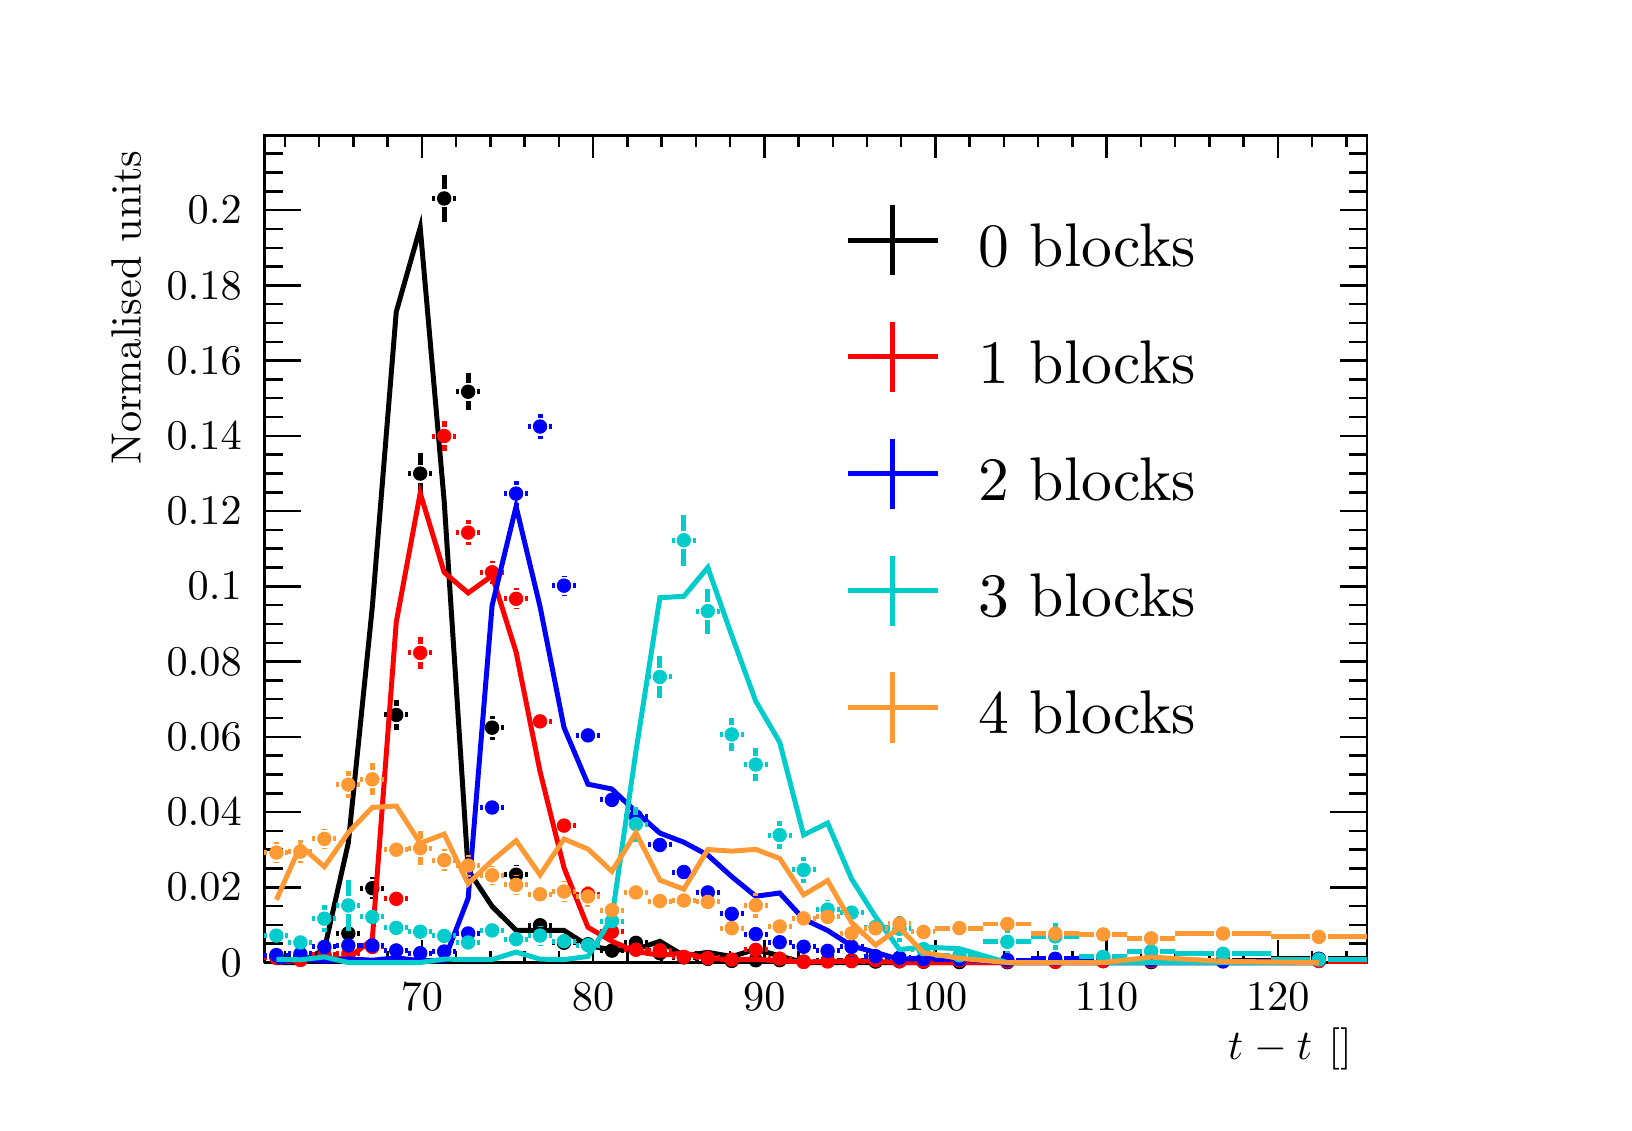
\begin{tikzpicture}
\pgfdeclareplotmark{cross} {
\pgfpathmoveto{\pgfpoint{-0.3\pgfplotmarksize}{\pgfplotmarksize}}
\pgfpathlineto{\pgfpoint{+0.3\pgfplotmarksize}{\pgfplotmarksize}}
\pgfpathlineto{\pgfpoint{+0.3\pgfplotmarksize}{0.3\pgfplotmarksize}}
\pgfpathlineto{\pgfpoint{+1\pgfplotmarksize}{0.3\pgfplotmarksize}}
\pgfpathlineto{\pgfpoint{+1\pgfplotmarksize}{-0.3\pgfplotmarksize}}
\pgfpathlineto{\pgfpoint{+0.3\pgfplotmarksize}{-0.3\pgfplotmarksize}}
\pgfpathlineto{\pgfpoint{+0.3\pgfplotmarksize}{-1.\pgfplotmarksize}}
\pgfpathlineto{\pgfpoint{-0.3\pgfplotmarksize}{-1.\pgfplotmarksize}}
\pgfpathlineto{\pgfpoint{-0.3\pgfplotmarksize}{-0.3\pgfplotmarksize}}
\pgfpathlineto{\pgfpoint{-1.\pgfplotmarksize}{-0.3\pgfplotmarksize}}
\pgfpathlineto{\pgfpoint{-1.\pgfplotmarksize}{0.3\pgfplotmarksize}}
\pgfpathlineto{\pgfpoint{-0.3\pgfplotmarksize}{0.3\pgfplotmarksize}}
\pgfpathclose
\pgfusepathqstroke
}
\pgfdeclareplotmark{cross*} {
\pgfpathmoveto{\pgfpoint{-0.3\pgfplotmarksize}{\pgfplotmarksize}}
\pgfpathlineto{\pgfpoint{+0.3\pgfplotmarksize}{\pgfplotmarksize}}
\pgfpathlineto{\pgfpoint{+0.3\pgfplotmarksize}{0.3\pgfplotmarksize}}
\pgfpathlineto{\pgfpoint{+1\pgfplotmarksize}{0.3\pgfplotmarksize}}
\pgfpathlineto{\pgfpoint{+1\pgfplotmarksize}{-0.3\pgfplotmarksize}}
\pgfpathlineto{\pgfpoint{+0.3\pgfplotmarksize}{-0.3\pgfplotmarksize}}
\pgfpathlineto{\pgfpoint{+0.3\pgfplotmarksize}{-1.\pgfplotmarksize}}
\pgfpathlineto{\pgfpoint{-0.3\pgfplotmarksize}{-1.\pgfplotmarksize}}
\pgfpathlineto{\pgfpoint{-0.3\pgfplotmarksize}{-0.3\pgfplotmarksize}}
\pgfpathlineto{\pgfpoint{-1.\pgfplotmarksize}{-0.3\pgfplotmarksize}}
\pgfpathlineto{\pgfpoint{-1.\pgfplotmarksize}{0.3\pgfplotmarksize}}
\pgfpathlineto{\pgfpoint{-0.3\pgfplotmarksize}{0.3\pgfplotmarksize}}
\pgfpathclose
\pgfusepathqfillstroke
}
\pgfdeclareplotmark{newstar} {
\pgfpathmoveto{\pgfqpoint{0pt}{\pgfplotmarksize}}
\pgfpathlineto{\pgfqpointpolar{44}{0.5\pgfplotmarksize}}
\pgfpathlineto{\pgfqpointpolar{18}{\pgfplotmarksize}}
\pgfpathlineto{\pgfqpointpolar{-20}{0.5\pgfplotmarksize}}
\pgfpathlineto{\pgfqpointpolar{-54}{\pgfplotmarksize}}
\pgfpathlineto{\pgfqpointpolar{-90}{0.5\pgfplotmarksize}}
\pgfpathlineto{\pgfqpointpolar{234}{\pgfplotmarksize}}
\pgfpathlineto{\pgfqpointpolar{198}{0.5\pgfplotmarksize}}
\pgfpathlineto{\pgfqpointpolar{162}{\pgfplotmarksize}}
\pgfpathlineto{\pgfqpointpolar{134}{0.5\pgfplotmarksize}}
\pgfpathclose
\pgfusepathqstroke
}
\pgfdeclareplotmark{newstar*} {
\pgfpathmoveto{\pgfqpoint{0pt}{\pgfplotmarksize}}
\pgfpathlineto{\pgfqpointpolar{44}{0.5\pgfplotmarksize}}
\pgfpathlineto{\pgfqpointpolar{18}{\pgfplotmarksize}}
\pgfpathlineto{\pgfqpointpolar{-20}{0.5\pgfplotmarksize}}
\pgfpathlineto{\pgfqpointpolar{-54}{\pgfplotmarksize}}
\pgfpathlineto{\pgfqpointpolar{-90}{0.5\pgfplotmarksize}}
\pgfpathlineto{\pgfqpointpolar{234}{\pgfplotmarksize}}
\pgfpathlineto{\pgfqpointpolar{198}{0.5\pgfplotmarksize}}
\pgfpathlineto{\pgfqpointpolar{162}{\pgfplotmarksize}}
\pgfpathlineto{\pgfqpointpolar{134}{0.5\pgfplotmarksize}}
\pgfpathclose
\pgfusepathqfillstroke
}
\definecolor{c}{rgb}{1,1,1};
\draw [color=c, fill=c] (0,0) rectangle (20,13.639);
\draw [color=c, fill=c] (3,1.77307) rectangle (17,12.2751);
\definecolor{c}{rgb}{0,0,0};
\draw [c,line width=0.9] (3,1.77307) -- (3,12.2751) -- (17,12.2751) -- (17,1.77307) -- (3,1.77307);
\definecolor{c}{rgb}{1,1,1};
\draw [color=c, fill=c] (3,1.77307) rectangle (17,12.2751);
\definecolor{c}{rgb}{0,0,0};
\draw [c,line width=0.9] (3,1.77307) -- (3,12.2751) -- (17,12.2751) -- (17,1.77307) -- (3,1.77307);
\draw [c,line width=1.8] (3,1.85058) -- (3.03756,1.85058);
\draw [c,line width=1.8] (3.26679,1.85058) -- (3.30435,1.85058);
\foreach \P in {(3.15217,1.85058)}{\draw[mark options={color=c,fill=c},mark size=2.402402pt,mark=*] plot coordinates {\P};}
\draw [c,line width=1.8] (3.30435,1.84454) -- (3.34191,1.84454);
\draw [c,line width=1.8] (3.57113,1.84454) -- (3.6087,1.84454);
\foreach \P in {(3.45652,1.84454)}{\draw[mark options={color=c,fill=c},mark size=2.402402pt,mark=*] plot coordinates {\P};}
\draw [c,line width=1.8] (3.6087,1.86413) -- (3.64626,1.86413);
\draw [c,line width=1.8] (3.87548,1.86413) -- (3.91304,1.86413);
\foreach \P in {(3.76087,1.86413)}{\draw[mark options={color=c,fill=c},mark size=2.402402pt,mark=*] plot coordinates {\P};}
\draw [c,line width=1.8] (3.91304,2.14336) -- (3.9506,2.14336);
\draw [c,line width=1.8] (4.17983,2.14336) -- (4.21739,2.14336);
\foreach \P in {(4.06522,2.14336)}{\draw[mark options={color=c,fill=c},mark size=2.402402pt,mark=*] plot coordinates {\P};}
\draw [c,line width=1.8] (4.36957,2.58187) -- (4.36957,2.60319);
\draw [c,line width=1.8] (4.36957,2.83242) -- (4.36957,2.85374);
\draw [c,line width=1.8] (4.21739,2.71781) -- (4.25495,2.71781);
\draw [c,line width=1.8] (4.48418,2.71781) -- (4.52174,2.71781);
\foreach \P in {(4.36957,2.71781)}{\draw[mark options={color=c,fill=c},mark size=2.402402pt,mark=*] plot coordinates {\P};}
\draw [c,line width=1.8] (4.67391,4.72246) -- (4.67391,4.80279);
\draw [c,line width=1.8] (4.67391,5.03202) -- (4.67391,5.11236);
\draw [c,line width=1.8] (4.52174,4.91741) -- (4.5593,4.91741);
\draw [c,line width=1.8] (4.78853,4.91741) -- (4.82609,4.91741);
\foreach \P in {(4.67391,4.91741)}{\draw[mark options={color=c,fill=c},mark size=2.402402pt,mark=*] plot coordinates {\P};}
\draw [c,line width=1.8] (4.97826,7.72664) -- (4.97826,7.86854);
\draw [c,line width=1.8] (4.97826,8.09777) -- (4.97826,8.23967);
\draw [c,line width=1.8] (4.82609,7.98316) -- (4.86365,7.98316);
\draw [c,line width=1.8] (5.09287,7.98316) -- (5.13043,7.98316);
\foreach \P in {(4.97826,7.98316)}{\draw[mark options={color=c,fill=c},mark size=2.402402pt,mark=*] plot coordinates {\P};}
\draw [c,line width=1.8] (5.28261,11.1788) -- (5.28261,11.3623);
\draw [c,line width=1.8] (5.28261,11.5915) -- (5.28261,11.775);
\draw [c,line width=1.8] (5.13043,11.4769) -- (5.168,11.4769);
\draw [c,line width=1.8] (5.39722,11.4769) -- (5.43478,11.4769);
\foreach \P in {(5.28261,11.4769)}{\draw[mark options={color=c,fill=c},mark size=2.402402pt,mark=*] plot coordinates {\P};}
\draw [c,line width=1.8] (5.58696,8.78629) -- (5.58696,8.90786);
\draw [c,line width=1.8] (5.58696,9.13708) -- (5.58696,9.25865);
\draw [c,line width=1.8] (5.43478,9.02247) -- (5.47234,9.02247);
\draw [c,line width=1.8] (5.70157,9.02247) -- (5.73913,9.02247);
\foreach \P in {(5.58696,9.02247)}{\draw[mark options={color=c,fill=c},mark size=2.402402pt,mark=*] plot coordinates {\P};}
\draw [c,line width=1.8] (5.8913,4.60254) -- (5.8913,4.64143);
\draw [c,line width=1.8] (5.8913,4.87066) -- (5.8913,4.90955);
\draw [c,line width=1.8] (5.73913,4.75604) -- (5.77669,4.75604);
\draw [c,line width=1.8] (6.00592,4.75604) -- (6.04348,4.75604);
\foreach \P in {(5.8913,4.75604)}{\draw[mark options={color=c,fill=c},mark size=2.402402pt,mark=*] plot coordinates {\P};}
\draw [c,line width=1.8] (6.19565,2.76179) -- (6.19565,2.77371);
\draw [c,line width=1.8] (6.19565,3.00294) -- (6.19565,3.01486);
\draw [c,line width=1.8] (6.04348,2.88833) -- (6.08104,2.88833);
\draw [c,line width=1.8] (6.31027,2.88833) -- (6.34783,2.88833);
\foreach \P in {(6.19565,2.88833)}{\draw[mark options={color=c,fill=c},mark size=2.402402pt,mark=*] plot coordinates {\P};}
\draw [c,line width=1.8] (6.34783,2.24704) -- (6.38539,2.24704);
\draw [c,line width=1.8] (6.61461,2.24704) -- (6.65217,2.24704);
\foreach \P in {(6.5,2.24704)}{\draw[mark options={color=c,fill=c},mark size=2.402402pt,mark=*] plot coordinates {\P};}
\draw [c,line width=1.8] (6.65217,2.02432) -- (6.68973,2.02432);
\draw [c,line width=1.8] (6.91896,2.02432) -- (6.95652,2.02432);
\foreach \P in {(6.80435,2.02432)}{\draw[mark options={color=c,fill=c},mark size=2.402402pt,mark=*] plot coordinates {\P};}
\draw [c,line width=1.8] (6.95652,2.00521) -- (6.99408,2.00521);
\draw [c,line width=1.8] (7.22331,2.00521) -- (7.26087,2.00521);
\foreach \P in {(7.1087,2.00521)}{\draw[mark options={color=c,fill=c},mark size=2.402402pt,mark=*] plot coordinates {\P};}
\draw [c,line width=1.8] (7.26087,1.92454) -- (7.29843,1.92454);
\draw [c,line width=1.8] (7.52766,1.92454) -- (7.56522,1.92454);
\foreach \P in {(7.41304,1.92454)}{\draw[mark options={color=c,fill=c},mark size=2.402402pt,mark=*] plot coordinates {\P};}
\draw [c,line width=1.8] (7.56522,2.02302) -- (7.60278,2.02302);
\draw [c,line width=1.8] (7.832,2.02302) -- (7.86957,2.02302);
\foreach \P in {(7.71739,2.02302)}{\draw[mark options={color=c,fill=c},mark size=2.402402pt,mark=*] plot coordinates {\P};}
\draw [c,line width=1.8] (7.86957,1.89203) -- (7.90713,1.89203);
\draw [c,line width=1.8] (8.13635,1.89203) -- (8.17391,1.89203);
\foreach \P in {(8.02174,1.89203)}{\draw[mark options={color=c,fill=c},mark size=2.402402pt,mark=*] plot coordinates {\P};}
\draw [c,line width=1.8] (8.17391,1.83837) -- (8.21147,1.83837);
\draw [c,line width=1.8] (8.4407,1.83837) -- (8.47826,1.83837);
\foreach \P in {(8.32609,1.83837)}{\draw[mark options={color=c,fill=c},mark size=2.402402pt,mark=*] plot coordinates {\P};}
\draw [c,line width=1.8] (8.47826,1.82007) -- (8.51582,1.82007);
\draw [c,line width=1.8] (8.74505,1.82007) -- (8.78261,1.82007);
\foreach \P in {(8.63043,1.82007)}{\draw[mark options={color=c,fill=c},mark size=2.402402pt,mark=*] plot coordinates {\P};}
\draw [c,line width=1.8] (8.78261,1.7937) -- (8.82017,1.7937);
\draw [c,line width=1.8] (9.0494,1.7937) -- (9.08696,1.7937);
\foreach \P in {(8.93478,1.7937)}{\draw[mark options={color=c,fill=c},mark size=2.402402pt,mark=*] plot coordinates {\P};}
\draw [c,line width=1.8] (9.08696,1.80199) -- (9.12452,1.80199);
\draw [c,line width=1.8] (9.35374,1.80199) -- (9.3913,1.80199);
\foreach \P in {(9.23913,1.80199)}{\draw[mark options={color=c,fill=c},mark size=2.402402pt,mark=*] plot coordinates {\P};}
\draw [c,line width=1.8] (9.3913,1.80382) -- (9.42887,1.80382);
\draw [c,line width=1.8] (9.65809,1.80382) -- (9.69565,1.80382);
\foreach \P in {(9.54348,1.80382)}{\draw[mark options={color=c,fill=c},mark size=2.402402pt,mark=*] plot coordinates {\P};}
\draw [c,line width=1.8] (9.69565,1.78407) -- (9.73321,1.78407);
\draw [c,line width=1.8] (9.96244,1.78407) -- (10,1.78407);
\foreach \P in {(9.84783,1.78407)}{\draw[mark options={color=c,fill=c},mark size=2.402402pt,mark=*] plot coordinates {\P};}
\draw [c,line width=1.8] (10,1.79748) -- (10.0376,1.79748);
\draw [c,line width=1.8] (10.2668,1.79748) -- (10.3043,1.79748);
\foreach \P in {(10.1522,1.79748)}{\draw[mark options={color=c,fill=c},mark size=2.402402pt,mark=*] plot coordinates {\P};}
\draw [c,line width=1.8] (10.3043,1.80015) -- (10.3419,1.80015);
\draw [c,line width=1.8] (10.5711,1.80015) -- (10.6087,1.80015);
\foreach \P in {(10.4565,1.80015)}{\draw[mark options={color=c,fill=c},mark size=2.402402pt,mark=*] plot coordinates {\P};}
\draw [c,line width=1.8] (10.6087,1.78576) -- (10.6463,1.78576);
\draw [c,line width=1.8] (10.8755,1.78576) -- (10.913,1.78576);
\foreach \P in {(10.7609,1.78576)}{\draw[mark options={color=c,fill=c},mark size=2.402402pt,mark=*] plot coordinates {\P};}
\draw [c,line width=1.8] (10.913,1.78885) -- (10.9506,1.78885);
\draw [c,line width=1.8] (11.1798,1.78885) -- (11.2174,1.78885);
\foreach \P in {(11.0652,1.78885)}{\draw[mark options={color=c,fill=c},mark size=2.402402pt,mark=*] plot coordinates {\P};}
\draw [c,line width=1.8] (11.2174,1.78321) -- (11.255,1.78321);
\draw [c,line width=1.8] (11.4842,1.78321) -- (11.5217,1.78321);
\foreach \P in {(11.3696,1.78321)}{\draw[mark options={color=c,fill=c},mark size=2.402402pt,mark=*] plot coordinates {\P};}
\draw [c,line width=1.8] (11.5217,1.77882) -- (11.7115,1.77882);
\draw [c,line width=1.8] (11.9407,1.77882) -- (12.1304,1.77882);
\foreach \P in {(11.8261,1.77882)}{\draw[mark options={color=c,fill=c},mark size=2.402402pt,mark=*] plot coordinates {\P};}
\draw [c,line width=1.8] (12.1304,1.77744) -- (12.3202,1.77744);
\draw [c,line width=1.8] (12.5494,1.77744) -- (12.7391,1.77744);
\foreach \P in {(12.4348,1.77744)}{\draw[mark options={color=c,fill=c},mark size=2.402402pt,mark=*] plot coordinates {\P};}
\draw [c,line width=1.8] (12.7391,1.79041) -- (12.9289,1.79041);
\draw [c,line width=1.8] (13.1581,1.79041) -- (13.3478,1.79041);
\foreach \P in {(13.0435,1.79041)}{\draw[mark options={color=c,fill=c},mark size=2.402402pt,mark=*] plot coordinates {\P};}
\draw [c,line width=1.8] (13.3478,1.79207) -- (13.5376,1.79207);
\draw [c,line width=1.8] (13.7668,1.79207) -- (13.9565,1.79207);
\foreach \P in {(13.6522,1.79207)}{\draw[mark options={color=c,fill=c},mark size=2.402402pt,mark=*] plot coordinates {\P};}
\draw [c,line width=1.8] (13.9565,1.77881) -- (14.1463,1.77881);
\draw [c,line width=1.8] (14.3755,1.77881) -- (14.5652,1.77881);
\foreach \P in {(14.2609,1.77881)}{\draw[mark options={color=c,fill=c},mark size=2.402402pt,mark=*] plot coordinates {\P};}
\draw [c,line width=1.8] (14.5652,1.79751) -- (15.0593,1.79751);
\draw [c,line width=1.8] (15.2885,1.79751) -- (15.7826,1.79751);
\foreach \P in {(15.1739,1.79751)}{\draw[mark options={color=c,fill=c},mark size=2.402402pt,mark=*] plot coordinates {\P};}
\draw [c,line width=1.8] (15.7826,1.82105) -- (16.2767,1.82105);
\draw [c,line width=1.8] (16.5059,1.82105) -- (17,1.82105);
\foreach \P in {(16.3913,1.82105)}{\draw[mark options={color=c,fill=c},mark size=2.402402pt,mark=*] plot coordinates {\P};}
\draw [c,line width=0.9] (3,1.77307) -- (17,1.77307);
\draw [c,line width=0.9] (5,2.05948) -- (5,1.77307);
\draw [c,line width=0.9] (5.43478,1.91628) -- (5.43478,1.77307);
\draw [c,line width=0.9] (5.86957,1.91628) -- (5.86957,1.77307);
\draw [c,line width=0.9] (6.30435,1.91628) -- (6.30435,1.77307);
\draw [c,line width=0.9] (6.73913,1.91628) -- (6.73913,1.77307);
\draw [c,line width=0.9] (7.17391,2.05948) -- (7.17391,1.77307);
\draw [c,line width=0.9] (7.6087,1.91628) -- (7.6087,1.77307);
\draw [c,line width=0.9] (8.04348,1.91628) -- (8.04348,1.77307);
\draw [c,line width=0.9] (8.47826,1.91628) -- (8.47826,1.77307);
\draw [c,line width=0.9] (8.91304,1.91628) -- (8.91304,1.77307);
\draw [c,line width=0.9] (9.34783,2.05948) -- (9.34783,1.77307);
\draw [c,line width=0.9] (9.78261,1.91628) -- (9.78261,1.77307);
\draw [c,line width=0.9] (10.2174,1.91628) -- (10.2174,1.77307);
\draw [c,line width=0.9] (10.6522,1.91628) -- (10.6522,1.77307);
\draw [c,line width=0.9] (11.087,1.91628) -- (11.087,1.77307);
\draw [c,line width=0.9] (11.5217,2.05948) -- (11.5217,1.77307);
\draw [c,line width=0.9] (11.9565,1.91628) -- (11.9565,1.77307);
\draw [c,line width=0.9] (12.3913,1.91628) -- (12.3913,1.77307);
\draw [c,line width=0.9] (12.8261,1.91628) -- (12.8261,1.77307);
\draw [c,line width=0.9] (13.2609,1.91628) -- (13.2609,1.77307);
\draw [c,line width=0.9] (13.6957,2.05948) -- (13.6957,1.77307);
\draw [c,line width=0.9] (14.1304,1.91628) -- (14.1304,1.77307);
\draw [c,line width=0.9] (14.5652,1.91628) -- (14.5652,1.77307);
\draw [c,line width=0.9] (15,1.91628) -- (15,1.77307);
\draw [c,line width=0.9] (15.4348,1.91628) -- (15.4348,1.77307);
\draw [c,line width=0.9] (15.8696,2.05948) -- (15.8696,1.77307);
\draw [c,line width=0.9] (5,2.05948) -- (5,1.77307);
\draw [c,line width=0.9] (4.56522,1.91628) -- (4.56522,1.77307);
\draw [c,line width=0.9] (4.13043,1.91628) -- (4.13043,1.77307);
\draw [c,line width=0.9] (3.69565,1.91628) -- (3.69565,1.77307);
\draw [c,line width=0.9] (3.26087,1.91628) -- (3.26087,1.77307);
\draw [c,line width=0.9] (15.8696,2.05948) -- (15.8696,1.77307);
\draw [c,line width=0.9] (16.3043,1.91628) -- (16.3043,1.77307);
\draw [c,line width=0.9] (16.7391,1.91628) -- (16.7391,1.77307);
\draw [anchor=base] (5,1.15931) node[scale=1.52731, color=c, rotate=0]{70};
\draw [anchor=base] (7.17391,1.15931) node[scale=1.52731, color=c, rotate=0]{80};
\draw [anchor=base] (9.34783,1.15931) node[scale=1.52731, color=c, rotate=0]{90};
\draw [anchor=base] (11.5217,1.15931) node[scale=1.52731, color=c, rotate=0]{100};
\draw [anchor=base] (13.6957,1.15931) node[scale=1.52731, color=c, rotate=0]{110};
\draw [anchor=base] (15.8696,1.15931) node[scale=1.52731, color=c, rotate=0]{120};
\draw [anchor= east] (17,0.681948) node[scale=1.52731, color=c, rotate=0]{$t_{\SFour} - t_{\STwo}$ [\si{\nano\second}] };
\draw [c,line width=0.9] (3,12.2751) -- (17,12.2751);
\draw [c,line width=0.9] (5,11.9887) -- (5,12.2751);
\draw [c,line width=0.9] (5.43478,12.1319) -- (5.43478,12.2751);
\draw [c,line width=0.9] (5.86957,12.1319) -- (5.86957,12.2751);
\draw [c,line width=0.9] (6.30435,12.1319) -- (6.30435,12.2751);
\draw [c,line width=0.9] (6.73913,12.1319) -- (6.73913,12.2751);
\draw [c,line width=0.9] (7.17391,11.9887) -- (7.17391,12.2751);
\draw [c,line width=0.9] (7.6087,12.1319) -- (7.6087,12.2751);
\draw [c,line width=0.9] (8.04348,12.1319) -- (8.04348,12.2751);
\draw [c,line width=0.9] (8.47826,12.1319) -- (8.47826,12.2751);
\draw [c,line width=0.9] (8.91304,12.1319) -- (8.91304,12.2751);
\draw [c,line width=0.9] (9.34783,11.9887) -- (9.34783,12.2751);
\draw [c,line width=0.9] (9.78261,12.1319) -- (9.78261,12.2751);
\draw [c,line width=0.9] (10.2174,12.1319) -- (10.2174,12.2751);
\draw [c,line width=0.9] (10.6522,12.1319) -- (10.6522,12.2751);
\draw [c,line width=0.9] (11.087,12.1319) -- (11.087,12.2751);
\draw [c,line width=0.9] (11.5217,11.9887) -- (11.5217,12.2751);
\draw [c,line width=0.9] (11.9565,12.1319) -- (11.9565,12.2751);
\draw [c,line width=0.9] (12.3913,12.1319) -- (12.3913,12.2751);
\draw [c,line width=0.9] (12.8261,12.1319) -- (12.8261,12.2751);
\draw [c,line width=0.9] (13.2609,12.1319) -- (13.2609,12.2751);
\draw [c,line width=0.9] (13.6957,11.9887) -- (13.6957,12.2751);
\draw [c,line width=0.9] (14.1304,12.1319) -- (14.1304,12.2751);
\draw [c,line width=0.9] (14.5652,12.1319) -- (14.5652,12.2751);
\draw [c,line width=0.9] (15,12.1319) -- (15,12.2751);
\draw [c,line width=0.9] (15.4348,12.1319) -- (15.4348,12.2751);
\draw [c,line width=0.9] (15.8696,11.9887) -- (15.8696,12.2751);
\draw [c,line width=0.9] (5,11.9887) -- (5,12.2751);
\draw [c,line width=0.9] (4.56522,12.1319) -- (4.56522,12.2751);
\draw [c,line width=0.9] (4.13043,12.1319) -- (4.13043,12.2751);
\draw [c,line width=0.9] (3.69565,12.1319) -- (3.69565,12.2751);
\draw [c,line width=0.9] (3.26087,12.1319) -- (3.26087,12.2751);
\draw [c,line width=0.9] (15.8696,11.9887) -- (15.8696,12.2751);
\draw [c,line width=0.9] (16.3043,12.1319) -- (16.3043,12.2751);
\draw [c,line width=0.9] (16.7391,12.1319) -- (16.7391,12.2751);
\draw [c,line width=0.9] (3,1.77307) -- (3,12.2751);
\draw [c,line width=0.9] (3.462,1.77307) -- (3,1.77307);
\draw [c,line width=0.9] (3.231,2.01195) -- (3,2.01195);
\draw [c,line width=0.9] (3.231,2.25084) -- (3,2.25084);
\draw [c,line width=0.9] (3.231,2.48973) -- (3,2.48973);
\draw [c,line width=0.9] (3.462,2.72861) -- (3,2.72861);
\draw [c,line width=0.9] (3.231,2.9675) -- (3,2.9675);
\draw [c,line width=0.9] (3.231,3.20638) -- (3,3.20638);
\draw [c,line width=0.9] (3.231,3.44527) -- (3,3.44527);
\draw [c,line width=0.9] (3.462,3.68416) -- (3,3.68416);
\draw [c,line width=0.9] (3.231,3.92304) -- (3,3.92304);
\draw [c,line width=0.9] (3.231,4.16193) -- (3,4.16193);
\draw [c,line width=0.9] (3.231,4.40082) -- (3,4.40082);
\draw [c,line width=0.9] (3.462,4.6397) -- (3,4.6397);
\draw [c,line width=0.9] (3.231,4.87859) -- (3,4.87859);
\draw [c,line width=0.9] (3.231,5.11748) -- (3,5.11748);
\draw [c,line width=0.9] (3.231,5.35636) -- (3,5.35636);
\draw [c,line width=0.9] (3.462,5.59525) -- (3,5.59525);
\draw [c,line width=0.9] (3.231,5.83414) -- (3,5.83414);
\draw [c,line width=0.9] (3.231,6.07302) -- (3,6.07302);
\draw [c,line width=0.9] (3.231,6.31191) -- (3,6.31191);
\draw [c,line width=0.9] (3.462,6.5508) -- (3,6.5508);
\draw [c,line width=0.9] (3.231,6.78968) -- (3,6.78968);
\draw [c,line width=0.9] (3.231,7.02857) -- (3,7.02857);
\draw [c,line width=0.9] (3.231,7.26746) -- (3,7.26746);
\draw [c,line width=0.9] (3.462,7.50634) -- (3,7.50634);
\draw [c,line width=0.9] (3.231,7.74523) -- (3,7.74523);
\draw [c,line width=0.9] (3.231,7.98412) -- (3,7.98412);
\draw [c,line width=0.9] (3.231,8.223) -- (3,8.223);
\draw [c,line width=0.9] (3.462,8.46189) -- (3,8.46189);
\draw [c,line width=0.9] (3.231,8.70078) -- (3,8.70078);
\draw [c,line width=0.9] (3.231,8.93966) -- (3,8.93966);
\draw [c,line width=0.9] (3.231,9.17855) -- (3,9.17855);
\draw [c,line width=0.9] (3.462,9.41743) -- (3,9.41743);
\draw [c,line width=0.9] (3.231,9.65632) -- (3,9.65632);
\draw [c,line width=0.9] (3.231,9.89521) -- (3,9.89521);
\draw [c,line width=0.9] (3.231,10.1341) -- (3,10.1341);
\draw [c,line width=0.9] (3.462,10.373) -- (3,10.373);
\draw [c,line width=0.9] (3.231,10.6119) -- (3,10.6119);
\draw [c,line width=0.9] (3.231,10.8508) -- (3,10.8508);
\draw [c,line width=0.9] (3.231,11.0896) -- (3,11.0896);
\draw [c,line width=0.9] (3.462,11.3285) -- (3,11.3285);
\draw [c,line width=0.9] (3.462,11.3285) -- (3,11.3285);
\draw [c,line width=0.9] (3.231,11.5674) -- (3,11.5674);
\draw [c,line width=0.9] (3.231,11.8063) -- (3,11.8063);
\draw [c,line width=0.9] (3.231,12.0452) -- (3,12.0452);
\draw [anchor= east] (2.9,1.77307) node[scale=1.52731, color=c, rotate=0]{0};
\draw [anchor= east] (2.9,2.72861) node[scale=1.52731, color=c, rotate=0]{0.02};
\draw [anchor= east] (2.9,3.68416) node[scale=1.52731, color=c, rotate=0]{0.04};
\draw [anchor= east] (2.9,4.6397) node[scale=1.52731, color=c, rotate=0]{0.06};
\draw [anchor= east] (2.9,5.59525) node[scale=1.52731, color=c, rotate=0]{0.08};
\draw [anchor= east] (2.9,6.5508) node[scale=1.52731, color=c, rotate=0]{0.1};
\draw [anchor= east] (2.9,7.50634) node[scale=1.52731, color=c, rotate=0]{0.12};
\draw [anchor= east] (2.9,8.46189) node[scale=1.52731, color=c, rotate=0]{0.14};
\draw [anchor= east] (2.9,9.41743) node[scale=1.52731, color=c, rotate=0]{0.16};
\draw [anchor= east] (2.9,10.373) node[scale=1.52731, color=c, rotate=0]{0.18};
\draw [anchor= east] (2.9,11.3285) node[scale=1.52731, color=c, rotate=0]{0.2};
\draw [anchor= east] (1.24,12.2751) node[scale=1.52731, color=c, rotate=90]{Normalised units};
\draw [c,line width=0.9] (17,1.77307) -- (17,12.2751);
\draw [c,line width=0.9] (16.538,1.77307) -- (17,1.77307);
\draw [c,line width=0.9] (16.769,2.01195) -- (17,2.01195);
\draw [c,line width=0.9] (16.769,2.25084) -- (17,2.25084);
\draw [c,line width=0.9] (16.769,2.48973) -- (17,2.48973);
\draw [c,line width=0.9] (16.538,2.72861) -- (17,2.72861);
\draw [c,line width=0.9] (16.769,2.9675) -- (17,2.9675);
\draw [c,line width=0.9] (16.769,3.20638) -- (17,3.20638);
\draw [c,line width=0.9] (16.769,3.44527) -- (17,3.44527);
\draw [c,line width=0.9] (16.538,3.68416) -- (17,3.68416);
\draw [c,line width=0.9] (16.769,3.92304) -- (17,3.92304);
\draw [c,line width=0.9] (16.769,4.16193) -- (17,4.16193);
\draw [c,line width=0.9] (16.769,4.40082) -- (17,4.40082);
\draw [c,line width=0.9] (16.538,4.6397) -- (17,4.6397);
\draw [c,line width=0.9] (16.769,4.87859) -- (17,4.87859);
\draw [c,line width=0.9] (16.769,5.11748) -- (17,5.11748);
\draw [c,line width=0.9] (16.769,5.35636) -- (17,5.35636);
\draw [c,line width=0.9] (16.538,5.59525) -- (17,5.59525);
\draw [c,line width=0.9] (16.769,5.83414) -- (17,5.83414);
\draw [c,line width=0.9] (16.769,6.07302) -- (17,6.07302);
\draw [c,line width=0.9] (16.769,6.31191) -- (17,6.31191);
\draw [c,line width=0.9] (16.538,6.5508) -- (17,6.5508);
\draw [c,line width=0.9] (16.769,6.78968) -- (17,6.78968);
\draw [c,line width=0.9] (16.769,7.02857) -- (17,7.02857);
\draw [c,line width=0.9] (16.769,7.26746) -- (17,7.26746);
\draw [c,line width=0.9] (16.538,7.50634) -- (17,7.50634);
\draw [c,line width=0.9] (16.769,7.74523) -- (17,7.74523);
\draw [c,line width=0.9] (16.769,7.98412) -- (17,7.98412);
\draw [c,line width=0.9] (16.769,8.223) -- (17,8.223);
\draw [c,line width=0.9] (16.538,8.46189) -- (17,8.46189);
\draw [c,line width=0.9] (16.769,8.70078) -- (17,8.70078);
\draw [c,line width=0.9] (16.769,8.93966) -- (17,8.93966);
\draw [c,line width=0.9] (16.769,9.17855) -- (17,9.17855);
\draw [c,line width=0.9] (16.538,9.41743) -- (17,9.41743);
\draw [c,line width=0.9] (16.769,9.65632) -- (17,9.65632);
\draw [c,line width=0.9] (16.769,9.89521) -- (17,9.89521);
\draw [c,line width=0.9] (16.769,10.1341) -- (17,10.1341);
\draw [c,line width=0.9] (16.538,10.373) -- (17,10.373);
\draw [c,line width=0.9] (16.769,10.6119) -- (17,10.6119);
\draw [c,line width=0.9] (16.769,10.8508) -- (17,10.8508);
\draw [c,line width=0.9] (16.769,11.0896) -- (17,11.0896);
\draw [c,line width=0.9] (16.538,11.3285) -- (17,11.3285);
\draw [c,line width=0.9] (16.538,11.3285) -- (17,11.3285);
\draw [c,line width=0.9] (16.769,11.5674) -- (17,11.5674);
\draw [c,line width=0.9] (16.769,11.8063) -- (17,11.8063);
\draw [c,line width=0.9] (16.769,12.0452) -- (17,12.0452);
\draw [c,line width=1.8] (3.15217,1.77307) -- (3.45652,1.77307) -- (3.76087,1.94001) -- (4.06522,3.29319) -- (4.36957,6.28525) -- (4.67391,10.0364) -- (4.97826,11.1069) -- (5.28261,7.63227) -- (5.58696,2.94725) -- (5.8913,2.48632) --
 (6.19565,2.18325) -- (6.5,2.1818) -- (6.80435,2.1805) -- (7.1087,1.9891) -- (7.41304,1.93382) -- (7.71739,1.93863) -- (8.02174,2.04269) -- (8.32609,1.8601) -- (8.63043,1.90255) -- (8.93478,1.8496) -- (9.23913,1.94098) -- (9.54348,1.85732) --
 (9.84783,1.77307) -- (10.1522,1.77307) -- (10.4565,1.77307) -- (10.7609,1.77307) -- (11.0652,1.77307) -- (11.3696,1.77307) -- (11.8261,1.77307) -- (12.4348,1.77307) -- (13.0435,1.77307) -- (13.6522,1.77307) -- (14.2609,1.77307) -- (15.1739,1.77307)
 -- (16.3913,1.77307);
\definecolor{c}{rgb}{1,0,0};
\draw [c,line width=1.8] (3,1.83134) -- (3.03756,1.83134);
\draw [c,line width=1.8] (3.26679,1.83134) -- (3.30435,1.83134);
\foreach \P in {(3.15217,1.83134)}{\draw[mark options={color=c,fill=c},mark size=2.402402pt,mark=*] plot coordinates {\P};}
\draw [c,line width=1.8] (3.30435,1.80544) -- (3.34191,1.80544);
\draw [c,line width=1.8] (3.57113,1.80544) -- (3.6087,1.80544);
\foreach \P in {(3.45652,1.80544)}{\draw[mark options={color=c,fill=c},mark size=2.402402pt,mark=*] plot coordinates {\P};}
\draw [c,line width=1.8] (3.6087,1.88136) -- (3.64626,1.88136);
\draw [c,line width=1.8] (3.87548,1.88136) -- (3.91304,1.88136);
\foreach \P in {(3.76087,1.88136)}{\draw[mark options={color=c,fill=c},mark size=2.402402pt,mark=*] plot coordinates {\P};}
\draw [c,line width=1.8] (3.91304,1.88375) -- (3.9506,1.88375);
\draw [c,line width=1.8] (4.17983,1.88375) -- (4.21739,1.88375);
\foreach \P in {(4.06522,1.88375)}{\draw[mark options={color=c,fill=c},mark size=2.402402pt,mark=*] plot coordinates {\P};}
\draw [c,line width=1.8] (4.21739,1.97078) -- (4.25495,1.97078);
\draw [c,line width=1.8] (4.48418,1.97078) -- (4.52174,1.97078);
\foreach \P in {(4.36957,1.97078)}{\draw[mark options={color=c,fill=c},mark size=2.402402pt,mark=*] plot coordinates {\P};}
\draw [c,line width=1.8] (4.52174,2.5821) -- (4.5593,2.5821);
\draw [c,line width=1.8] (4.78853,2.5821) -- (4.82609,2.5821);
\foreach \P in {(4.67391,2.5821)}{\draw[mark options={color=c,fill=c},mark size=2.402402pt,mark=*] plot coordinates {\P};}
\draw [c,line width=1.8] (4.97826,5.50316) -- (4.97826,5.59138);
\draw [c,line width=1.8] (4.97826,5.82061) -- (4.97826,5.90883);
\draw [c,line width=1.8] (4.82609,5.70599) -- (4.86365,5.70599);
\draw [c,line width=1.8] (5.09287,5.70599) -- (5.13043,5.70599);
\foreach \P in {(4.97826,5.70599)}{\draw[mark options={color=c,fill=c},mark size=2.402402pt,mark=*] plot coordinates {\P};}
\draw [c,line width=1.8] (5.28261,8.2737) -- (5.28261,8.34535);
\draw [c,line width=1.8] (5.28261,8.57458) -- (5.28261,8.64623);
\draw [c,line width=1.8] (5.13043,8.45997) -- (5.168,8.45997);
\draw [c,line width=1.8] (5.39722,8.45997) -- (5.43478,8.45997);
\foreach \P in {(5.28261,8.45997)}{\draw[mark options={color=c,fill=c},mark size=2.402402pt,mark=*] plot coordinates {\P};}
\draw [c,line width=1.8] (5.58696,7.07052) -- (5.58696,7.1183);
\draw [c,line width=1.8] (5.58696,7.34753) -- (5.58696,7.3953);
\draw [c,line width=1.8] (5.43478,7.23291) -- (5.47234,7.23291);
\draw [c,line width=1.8] (5.70157,7.23291) -- (5.73913,7.23291);
\foreach \P in {(5.58696,7.23291)}{\draw[mark options={color=c,fill=c},mark size=2.402402pt,mark=*] plot coordinates {\P};}
\draw [c,line width=1.8] (5.8913,6.58057) -- (5.8913,6.61441);
\draw [c,line width=1.8] (5.8913,6.84363) -- (5.8913,6.87748);
\draw [c,line width=1.8] (5.73913,6.72902) -- (5.77669,6.72902);
\draw [c,line width=1.8] (6.00592,6.72902) -- (6.04348,6.72902);
\foreach \P in {(5.8913,6.72902)}{\draw[mark options={color=c,fill=c},mark size=2.402402pt,mark=*] plot coordinates {\P};}
\draw [c,line width=1.8] (6.19565,6.25738) -- (6.19565,6.27737);
\draw [c,line width=1.8] (6.19565,6.5066) -- (6.19565,6.52659);
\draw [c,line width=1.8] (6.04348,6.39198) -- (6.08104,6.39198);
\draw [c,line width=1.8] (6.31027,6.39198) -- (6.34783,6.39198);
\foreach \P in {(6.19565,6.39198)}{\draw[mark options={color=c,fill=c},mark size=2.402402pt,mark=*] plot coordinates {\P};}
\draw [c,line width=1.8] (6.34783,4.83602) -- (6.38539,4.83602);
\draw [c,line width=1.8] (6.61461,4.83602) -- (6.65217,4.83602);
\foreach \P in {(6.5,4.83602)}{\draw[mark options={color=c,fill=c},mark size=2.402402pt,mark=*] plot coordinates {\P};}
\draw [c,line width=1.8] (6.65217,3.51237) -- (6.68973,3.51237);
\draw [c,line width=1.8] (6.91896,3.51237) -- (6.95652,3.51237);
\foreach \P in {(6.80435,3.51237)}{\draw[mark options={color=c,fill=c},mark size=2.402402pt,mark=*] plot coordinates {\P};}
\draw [c,line width=1.8] (6.95652,2.64336) -- (6.99408,2.64336);
\draw [c,line width=1.8] (7.22331,2.64336) -- (7.26087,2.64336);
\foreach \P in {(7.1087,2.64336)}{\draw[mark options={color=c,fill=c},mark size=2.402402pt,mark=*] plot coordinates {\P};}
\draw [c,line width=1.8] (7.26087,2.16376) -- (7.29843,2.16376);
\draw [c,line width=1.8] (7.52766,2.16376) -- (7.56522,2.16376);
\foreach \P in {(7.41304,2.16376)}{\draw[mark options={color=c,fill=c},mark size=2.402402pt,mark=*] plot coordinates {\P};}
\draw [c,line width=1.8] (7.56522,1.93516) -- (7.60278,1.93516);
\draw [c,line width=1.8] (7.832,1.93516) -- (7.86957,1.93516);
\foreach \P in {(7.71739,1.93516)}{\draw[mark options={color=c,fill=c},mark size=2.402402pt,mark=*] plot coordinates {\P};}
\draw [c,line width=1.8] (7.86957,1.92811) -- (7.90713,1.92811);
\draw [c,line width=1.8] (8.13635,1.92811) -- (8.17391,1.92811);
\foreach \P in {(8.02174,1.92811)}{\draw[mark options={color=c,fill=c},mark size=2.402402pt,mark=*] plot coordinates {\P};}
\draw [c,line width=1.8] (8.17391,1.84466) -- (8.21147,1.84466);
\draw [c,line width=1.8] (8.4407,1.84466) -- (8.47826,1.84466);
\foreach \P in {(8.32609,1.84466)}{\draw[mark options={color=c,fill=c},mark size=2.402402pt,mark=*] plot coordinates {\P};}
\draw [c,line width=1.8] (8.47826,1.83124) -- (8.51582,1.83124);
\draw [c,line width=1.8] (8.74505,1.83124) -- (8.78261,1.83124);
\foreach \P in {(8.63043,1.83124)}{\draw[mark options={color=c,fill=c},mark size=2.402402pt,mark=*] plot coordinates {\P};}
\draw [c,line width=1.8] (8.78261,1.81124) -- (8.82017,1.81124);
\draw [c,line width=1.8] (9.0494,1.81124) -- (9.08696,1.81124);
\foreach \P in {(8.93478,1.81124)}{\draw[mark options={color=c,fill=c},mark size=2.402402pt,mark=*] plot coordinates {\P};}
\draw [c,line width=1.8] (9.08696,1.93362) -- (9.12452,1.93362);
\draw [c,line width=1.8] (9.35374,1.93362) -- (9.3913,1.93362);
\foreach \P in {(9.23913,1.93362)}{\draw[mark options={color=c,fill=c},mark size=2.402402pt,mark=*] plot coordinates {\P};}
\draw [c,line width=1.8] (9.3913,1.82349) -- (9.42887,1.82349);
\draw [c,line width=1.8] (9.65809,1.82349) -- (9.69565,1.82349);
\foreach \P in {(9.54348,1.82349)}{\draw[mark options={color=c,fill=c},mark size=2.402402pt,mark=*] plot coordinates {\P};}
\draw [c,line width=1.8] (9.69565,1.78215) -- (9.73321,1.78215);
\draw [c,line width=1.8] (9.96244,1.78215) -- (10,1.78215);
\foreach \P in {(9.84783,1.78215)}{\draw[mark options={color=c,fill=c},mark size=2.402402pt,mark=*] plot coordinates {\P};}
\draw [c,line width=1.8] (10,1.7863) -- (10.0376,1.7863);
\draw [c,line width=1.8] (10.2668,1.7863) -- (10.3043,1.7863);
\foreach \P in {(10.1522,1.7863)}{\draw[mark options={color=c,fill=c},mark size=2.402402pt,mark=*] plot coordinates {\P};}
\draw [c,line width=1.8] (10.3043,1.79102) -- (10.3419,1.79102);
\draw [c,line width=1.8] (10.5711,1.79102) -- (10.6087,1.79102);
\foreach \P in {(10.4565,1.79102)}{\draw[mark options={color=c,fill=c},mark size=2.402402pt,mark=*] plot coordinates {\P};}
\draw [c,line width=1.8] (10.6087,1.80395) -- (10.6463,1.80395);
\draw [c,line width=1.8] (10.8755,1.80395) -- (10.913,1.80395);
\foreach \P in {(10.7609,1.80395)}{\draw[mark options={color=c,fill=c},mark size=2.402402pt,mark=*] plot coordinates {\P};}
\draw [c,line width=1.8] (10.913,1.79161) -- (10.9506,1.79161);
\draw [c,line width=1.8] (11.1798,1.79161) -- (11.2174,1.79161);
\foreach \P in {(11.0652,1.79161)}{\draw[mark options={color=c,fill=c},mark size=2.402402pt,mark=*] plot coordinates {\P};}
\draw [c,line width=1.8] (11.2174,1.78604) -- (11.255,1.78604);
\draw [c,line width=1.8] (11.4842,1.78604) -- (11.5217,1.78604);
\foreach \P in {(11.3696,1.78604)}{\draw[mark options={color=c,fill=c},mark size=2.402402pt,mark=*] plot coordinates {\P};}
\draw [c,line width=1.8] (11.5217,1.80082) -- (11.7115,1.80082);
\draw [c,line width=1.8] (11.9407,1.80082) -- (12.1304,1.80082);
\foreach \P in {(11.8261,1.80082)}{\draw[mark options={color=c,fill=c},mark size=2.402402pt,mark=*] plot coordinates {\P};}
\draw [c,line width=1.8] (12.1304,1.78662) -- (12.3202,1.78662);
\draw [c,line width=1.8] (12.5494,1.78662) -- (12.7391,1.78662);
\foreach \P in {(12.4348,1.78662)}{\draw[mark options={color=c,fill=c},mark size=2.402402pt,mark=*] plot coordinates {\P};}
\draw [c,line width=1.8] (12.7391,1.78028) -- (12.9289,1.78028);
\draw [c,line width=1.8] (13.1581,1.78028) -- (13.3478,1.78028);
\foreach \P in {(13.0435,1.78028)}{\draw[mark options={color=c,fill=c},mark size=2.402402pt,mark=*] plot coordinates {\P};}
\draw [c,line width=1.8] (13.3478,1.79188) -- (13.5376,1.79188);
\draw [c,line width=1.8] (13.7668,1.79188) -- (13.9565,1.79188);
\foreach \P in {(13.6522,1.79188)}{\draw[mark options={color=c,fill=c},mark size=2.402402pt,mark=*] plot coordinates {\P};}
\draw [c,line width=1.8] (13.9565,1.78931) -- (14.1463,1.78931);
\draw [c,line width=1.8] (14.3755,1.78931) -- (14.5652,1.78931);
\foreach \P in {(14.2609,1.78931)}{\draw[mark options={color=c,fill=c},mark size=2.402402pt,mark=*] plot coordinates {\P};}
\draw [c,line width=1.8] (14.5652,1.78607) -- (15.0593,1.78607);
\draw [c,line width=1.8] (15.2885,1.78607) -- (15.7826,1.78607);
\foreach \P in {(15.1739,1.78607)}{\draw[mark options={color=c,fill=c},mark size=2.402402pt,mark=*] plot coordinates {\P};}
\draw [c,line width=1.8] (15.7826,1.79171) -- (16.2767,1.79171);
\draw [c,line width=1.8] (16.5059,1.79171) -- (17,1.79171);
\foreach \P in {(16.3913,1.79171)}{\draw[mark options={color=c,fill=c},mark size=2.402402pt,mark=*] plot coordinates {\P};}
\draw [c,line width=1.8] (3.15217,1.77307) -- (3.45652,1.80439) -- (3.76087,1.81824) -- (4.06522,1.82878) -- (4.36957,2.06592) -- (4.67391,6.09562) -- (4.97826,7.73532) -- (5.28261,6.7284) -- (5.58696,6.46755) -- (5.8913,6.68629) -- (6.19565,5.71682)
 -- (6.5,4.19816) -- (6.80435,2.97689) -- (7.1087,2.22068) -- (7.41304,2.04275) -- (7.71739,1.91352) -- (8.02174,1.86436) -- (8.32609,1.89469) -- (8.63043,1.82614) -- (8.93478,1.80975) -- (9.23913,1.81482) -- (9.54348,1.79432) -- (9.84783,1.78204) --
 (10.1522,1.78366) -- (10.4565,1.79639) -- (10.7609,1.78777) -- (11.0652,1.77307) -- (11.3696,1.77307) -- (11.8261,1.77307) -- (12.4348,1.77307) -- (13.0435,1.77307) -- (13.6522,1.77307) -- (14.2609,1.77307) -- (15.1739,1.77307) -- (16.3913,1.77307);
\definecolor{c}{rgb}{0,0,1};
\draw [c,line width=1.8] (3,1.86742) -- (3.03756,1.86742);
\draw [c,line width=1.8] (3.26679,1.86742) -- (3.30435,1.86742);
\foreach \P in {(3.15217,1.86742)}{\draw[mark options={color=c,fill=c},mark size=2.402402pt,mark=*] plot coordinates {\P};}
\draw [c,line width=1.8] (3.30435,1.8819) -- (3.34191,1.8819);
\draw [c,line width=1.8] (3.57113,1.8819) -- (3.6087,1.8819);
\foreach \P in {(3.45652,1.8819)}{\draw[mark options={color=c,fill=c},mark size=2.402402pt,mark=*] plot coordinates {\P};}
\draw [c,line width=1.8] (3.6087,1.97196) -- (3.64626,1.97196);
\draw [c,line width=1.8] (3.87548,1.97196) -- (3.91304,1.97196);
\foreach \P in {(3.76087,1.97196)}{\draw[mark options={color=c,fill=c},mark size=2.402402pt,mark=*] plot coordinates {\P};}
\draw [c,line width=1.8] (3.91304,1.9899) -- (3.9506,1.9899);
\draw [c,line width=1.8] (4.17983,1.9899) -- (4.21739,1.9899);
\foreach \P in {(4.06522,1.9899)}{\draw[mark options={color=c,fill=c},mark size=2.402402pt,mark=*] plot coordinates {\P};}
\draw [c,line width=1.8] (4.21739,1.99006) -- (4.25495,1.99006);
\draw [c,line width=1.8] (4.48418,1.99006) -- (4.52174,1.99006);
\foreach \P in {(4.36957,1.99006)}{\draw[mark options={color=c,fill=c},mark size=2.402402pt,mark=*] plot coordinates {\P};}
\draw [c,line width=1.8] (4.52174,1.92687) -- (4.5593,1.92687);
\draw [c,line width=1.8] (4.78853,1.92687) -- (4.82609,1.92687);
\foreach \P in {(4.67391,1.92687)}{\draw[mark options={color=c,fill=c},mark size=2.402402pt,mark=*] plot coordinates {\P};}
\draw [c,line width=1.8] (4.82609,1.89187) -- (4.86365,1.89187);
\draw [c,line width=1.8] (5.09287,1.89187) -- (5.13043,1.89187);
\foreach \P in {(4.97826,1.89187)}{\draw[mark options={color=c,fill=c},mark size=2.402402pt,mark=*] plot coordinates {\P};}
\draw [c,line width=1.8] (5.13043,1.91297) -- (5.168,1.91297);
\draw [c,line width=1.8] (5.39722,1.91297) -- (5.43478,1.91297);
\foreach \P in {(5.28261,1.91297)}{\draw[mark options={color=c,fill=c},mark size=2.402402pt,mark=*] plot coordinates {\P};}
\draw [c,line width=1.8] (5.43478,2.14228) -- (5.47234,2.14228);
\draw [c,line width=1.8] (5.70157,2.14228) -- (5.73913,2.14228);
\foreach \P in {(5.58696,2.14228)}{\draw[mark options={color=c,fill=c},mark size=2.402402pt,mark=*] plot coordinates {\P};}
\draw [c,line width=1.8] (5.73913,3.74212) -- (5.77669,3.74212);
\draw [c,line width=1.8] (6.00592,3.74212) -- (6.04348,3.74212);
\foreach \P in {(5.8913,3.74212)}{\draw[mark options={color=c,fill=c},mark size=2.402402pt,mark=*] plot coordinates {\P};}
\draw [c,line width=1.8] (6.19565,7.57228) -- (6.19565,7.61454);
\draw [c,line width=1.8] (6.19565,7.84376) -- (6.19565,7.88602);
\draw [c,line width=1.8] (6.04348,7.72915) -- (6.08104,7.72915);
\draw [c,line width=1.8] (6.31027,7.72915) -- (6.34783,7.72915);
\foreach \P in {(6.19565,7.72915)}{\draw[mark options={color=c,fill=c},mark size=2.402402pt,mark=*] plot coordinates {\P};}
\draw [c,line width=1.8] (6.5,8.42446) -- (6.5,8.46571);
\draw [c,line width=1.8] (6.5,8.69493) -- (6.5,8.73619);
\draw [c,line width=1.8] (6.34783,8.58032) -- (6.38539,8.58032);
\draw [c,line width=1.8] (6.61461,8.58032) -- (6.65217,8.58032);
\foreach \P in {(6.5,8.58032)}{\draw[mark options={color=c,fill=c},mark size=2.402402pt,mark=*] plot coordinates {\P};}
\draw [c,line width=1.8] (6.80435,6.43707) -- (6.80435,6.44514);
\draw [c,line width=1.8] (6.80435,6.67437) -- (6.80435,6.68244);
\draw [c,line width=1.8] (6.65217,6.55975) -- (6.68973,6.55975);
\draw [c,line width=1.8] (6.91896,6.55975) -- (6.95652,6.55975);
\foreach \P in {(6.80435,6.55975)}{\draw[mark options={color=c,fill=c},mark size=2.402402pt,mark=*] plot coordinates {\P};}
\draw [c,line width=1.8] (6.95652,4.65795) -- (6.99408,4.65795);
\draw [c,line width=1.8] (7.22331,4.65795) -- (7.26087,4.65795);
\foreach \P in {(7.1087,4.65795)}{\draw[mark options={color=c,fill=c},mark size=2.402402pt,mark=*] plot coordinates {\P};}
\draw [c,line width=1.8] (7.26087,3.8386) -- (7.29843,3.8386);
\draw [c,line width=1.8] (7.52766,3.8386) -- (7.56522,3.8386);
\foreach \P in {(7.41304,3.8386)}{\draw[mark options={color=c,fill=c},mark size=2.402402pt,mark=*] plot coordinates {\P};}
\draw [c,line width=1.8] (7.56522,3.62833) -- (7.60278,3.62833);
\draw [c,line width=1.8] (7.832,3.62833) -- (7.86957,3.62833);
\foreach \P in {(7.71739,3.62833)}{\draw[mark options={color=c,fill=c},mark size=2.402402pt,mark=*] plot coordinates {\P};}
\draw [c,line width=1.8] (7.86957,3.26629) -- (7.90713,3.26629);
\draw [c,line width=1.8] (8.13635,3.26629) -- (8.17391,3.26629);
\foreach \P in {(8.02174,3.26629)}{\draw[mark options={color=c,fill=c},mark size=2.402402pt,mark=*] plot coordinates {\P};}
\draw [c,line width=1.8] (8.17391,2.92282) -- (8.21147,2.92282);
\draw [c,line width=1.8] (8.4407,2.92282) -- (8.47826,2.92282);
\foreach \P in {(8.32609,2.92282)}{\draw[mark options={color=c,fill=c},mark size=2.402402pt,mark=*] plot coordinates {\P};}
\draw [c,line width=1.8] (8.47826,2.66379) -- (8.51582,2.66379);
\draw [c,line width=1.8] (8.74505,2.66379) -- (8.78261,2.66379);
\foreach \P in {(8.63043,2.66379)}{\draw[mark options={color=c,fill=c},mark size=2.402402pt,mark=*] plot coordinates {\P};}
\draw [c,line width=1.8] (8.78261,2.39155) -- (8.82017,2.39155);
\draw [c,line width=1.8] (9.0494,2.39155) -- (9.08696,2.39155);
\foreach \P in {(8.93478,2.39155)}{\draw[mark options={color=c,fill=c},mark size=2.402402pt,mark=*] plot coordinates {\P};}
\draw [c,line width=1.8] (9.08696,2.13493) -- (9.12452,2.13493);
\draw [c,line width=1.8] (9.35374,2.13493) -- (9.3913,2.13493);
\foreach \P in {(9.23913,2.13493)}{\draw[mark options={color=c,fill=c},mark size=2.402402pt,mark=*] plot coordinates {\P};}
\draw [c,line width=1.8] (9.3913,2.03128) -- (9.42887,2.03128);
\draw [c,line width=1.8] (9.65809,2.03128) -- (9.69565,2.03128);
\foreach \P in {(9.54348,2.03128)}{\draw[mark options={color=c,fill=c},mark size=2.402402pt,mark=*] plot coordinates {\P};}
\draw [c,line width=1.8] (9.69565,1.97389) -- (9.73321,1.97389);
\draw [c,line width=1.8] (9.96244,1.97389) -- (10,1.97389);
\foreach \P in {(9.84783,1.97389)}{\draw[mark options={color=c,fill=c},mark size=2.402402pt,mark=*] plot coordinates {\P};}
\draw [c,line width=1.8] (10,1.92101) -- (10.0376,1.92101);
\draw [c,line width=1.8] (10.2668,1.92101) -- (10.3043,1.92101);
\foreach \P in {(10.1522,1.92101)}{\draw[mark options={color=c,fill=c},mark size=2.402402pt,mark=*] plot coordinates {\P};}
\draw [c,line width=1.8] (10.4565,1.85624) -- (10.4565,1.85816);
\draw [c,line width=1.8] (10.4565,2.08739) -- (10.4565,2.0893);
\draw [c,line width=1.8] (10.3043,1.97277) -- (10.3419,1.97277);
\draw [c,line width=1.8] (10.5711,1.97277) -- (10.6087,1.97277);
\foreach \P in {(10.4565,1.97277)}{\draw[mark options={color=c,fill=c},mark size=2.402402pt,mark=*] plot coordinates {\P};}
\draw [c,line width=1.8] (10.6087,1.85367) -- (10.6463,1.85367);
\draw [c,line width=1.8] (10.8755,1.85367) -- (10.913,1.85367);
\foreach \P in {(10.7609,1.85367)}{\draw[mark options={color=c,fill=c},mark size=2.402402pt,mark=*] plot coordinates {\P};}
\draw [c,line width=1.8] (10.913,1.83471) -- (10.9506,1.83471);
\draw [c,line width=1.8] (11.1798,1.83471) -- (11.2174,1.83471);
\foreach \P in {(11.0652,1.83471)}{\draw[mark options={color=c,fill=c},mark size=2.402402pt,mark=*] plot coordinates {\P};}
\draw [c,line width=1.8] (11.2174,1.81636) -- (11.255,1.81636);
\draw [c,line width=1.8] (11.4842,1.81636) -- (11.5217,1.81636);
\foreach \P in {(11.3696,1.81636)}{\draw[mark options={color=c,fill=c},mark size=2.402402pt,mark=*] plot coordinates {\P};}
\draw [c,line width=1.8] (11.5217,1.81554) -- (11.7115,1.81554);
\draw [c,line width=1.8] (11.9407,1.81554) -- (12.1304,1.81554);
\foreach \P in {(11.8261,1.81554)}{\draw[mark options={color=c,fill=c},mark size=2.402402pt,mark=*] plot coordinates {\P};}
\draw [c,line width=1.8] (12.1304,1.80386) -- (12.3202,1.80386);
\draw [c,line width=1.8] (12.5494,1.80386) -- (12.7391,1.80386);
\foreach \P in {(12.4348,1.80386)}{\draw[mark options={color=c,fill=c},mark size=2.402402pt,mark=*] plot coordinates {\P};}
\draw [c,line width=1.8] (12.7391,1.82091) -- (12.9289,1.82091);
\draw [c,line width=1.8] (13.1581,1.82091) -- (13.3478,1.82091);
\foreach \P in {(13.0435,1.82091)}{\draw[mark options={color=c,fill=c},mark size=2.402402pt,mark=*] plot coordinates {\P};}
\draw [c,line width=1.8] (13.3478,1.83547) -- (13.5376,1.83547);
\draw [c,line width=1.8] (13.7668,1.83547) -- (13.9565,1.83547);
\foreach \P in {(13.6522,1.83547)}{\draw[mark options={color=c,fill=c},mark size=2.402402pt,mark=*] plot coordinates {\P};}
\draw [c,line width=1.8] (13.9565,1.80422) -- (14.1463,1.80422);
\draw [c,line width=1.8] (14.3755,1.80422) -- (14.5652,1.80422);
\foreach \P in {(14.2609,1.80422)}{\draw[mark options={color=c,fill=c},mark size=2.402402pt,mark=*] plot coordinates {\P};}
\draw [c,line width=1.8] (14.5652,1.79187) -- (15.0593,1.79187);
\draw [c,line width=1.8] (15.2885,1.79187) -- (15.7826,1.79187);
\foreach \P in {(15.1739,1.79187)}{\draw[mark options={color=c,fill=c},mark size=2.402402pt,mark=*] plot coordinates {\P};}
\draw [c,line width=1.8] (15.7826,1.81642) -- (16.2767,1.81642);
\draw [c,line width=1.8] (16.5059,1.81642) -- (17,1.81642);
\foreach \P in {(16.3913,1.81642)}{\draw[mark options={color=c,fill=c},mark size=2.402402pt,mark=*] plot coordinates {\P};}
\draw [c,line width=1.8] (3.15217,1.77307) -- (3.45652,1.82502) -- (3.76087,1.79187) -- (4.06522,1.82042) -- (4.36957,1.80228) -- (4.67391,1.8328) -- (4.97826,1.79625) -- (5.28261,1.80039) -- (5.58696,2.58901) -- (5.8913,6.30856) -- (6.19565,7.56487)
 -- (6.5,6.2939) -- (6.80435,4.75839) -- (7.1087,4.03782) -- (7.41304,3.9769) -- (7.71739,3.68714) -- (8.02174,3.41704) -- (8.32609,3.30102) -- (8.63043,3.13769) -- (8.93478,2.8642) -- (9.23913,2.61487) -- (9.54348,2.65629) -- (9.84783,2.32483) --
 (10.1522,2.18005) -- (10.4565,1.98515) -- (10.7609,1.90177) -- (11.0652,1.81318) -- (11.3696,1.83151) -- (11.8261,1.81617) -- (12.4348,1.77307) -- (13.0435,1.77307) -- (13.6522,1.77307) -- (14.2609,1.77307) -- (15.1739,1.77307) -- (16.3913,1.77307);
\definecolor{c}{rgb}{0,0.8,0.8};
\draw [c,line width=1.8] (3,2.11499) -- (3.03756,2.11499);
\draw [c,line width=1.8] (3.26679,2.11499) -- (3.30435,2.11499);
\foreach \P in {(3.15217,2.11499)}{\draw[mark options={color=c,fill=c},mark size=2.402402pt,mark=*] plot coordinates {\P};}
\draw [c,line width=1.8] (3.30435,2.02817) -- (3.34191,2.02817);
\draw [c,line width=1.8] (3.57113,2.02817) -- (3.6087,2.02817);
\foreach \P in {(3.45652,2.02817)}{\draw[mark options={color=c,fill=c},mark size=2.402402pt,mark=*] plot coordinates {\P};}
\draw [c,line width=1.8] (3.76087,2.16229) -- (3.76087,2.21575);
\draw [c,line width=1.8] (3.76087,2.44498) -- (3.76087,2.49844);
\draw [c,line width=1.8] (3.6087,2.33037) -- (3.64626,2.33037);
\draw [c,line width=1.8] (3.87548,2.33037) -- (3.91304,2.33037);
\foreach \P in {(3.76087,2.33037)}{\draw[mark options={color=c,fill=c},mark size=2.402402pt,mark=*] plot coordinates {\P};}
\draw [c,line width=1.8] (4.06522,2.17513) -- (4.06522,2.3837);
\draw [c,line width=1.8] (4.06522,2.61292) -- (4.06522,2.82149);
\draw [c,line width=1.8] (3.91304,2.49831) -- (3.9506,2.49831);
\draw [c,line width=1.8] (4.17983,2.49831) -- (4.21739,2.49831);
\foreach \P in {(4.06522,2.49831)}{\draw[mark options={color=c,fill=c},mark size=2.402402pt,mark=*] plot coordinates {\P};}
\draw [c,line width=1.8] (4.21739,2.35186) -- (4.25495,2.35186);
\draw [c,line width=1.8] (4.48418,2.35186) -- (4.52174,2.35186);
\foreach \P in {(4.36957,2.35186)}{\draw[mark options={color=c,fill=c},mark size=2.402402pt,mark=*] plot coordinates {\P};}
\draw [c,line width=1.8] (4.52174,2.21293) -- (4.5593,2.21293);
\draw [c,line width=1.8] (4.78853,2.21293) -- (4.82609,2.21293);
\foreach \P in {(4.67391,2.21293)}{\draw[mark options={color=c,fill=c},mark size=2.402402pt,mark=*] plot coordinates {\P};}
\draw [c,line width=1.8] (4.82609,2.16525) -- (4.86365,2.16525);
\draw [c,line width=1.8] (5.09287,2.16525) -- (5.13043,2.16525);
\foreach \P in {(4.97826,2.16525)}{\draw[mark options={color=c,fill=c},mark size=2.402402pt,mark=*] plot coordinates {\P};}
\draw [c,line width=1.8] (5.13043,2.11104) -- (5.168,2.11104);
\draw [c,line width=1.8] (5.39722,2.11104) -- (5.43478,2.11104);
\foreach \P in {(5.28261,2.11104)}{\draw[mark options={color=c,fill=c},mark size=2.402402pt,mark=*] plot coordinates {\P};}
\draw [c,line width=1.8] (5.43478,2.02794) -- (5.47234,2.02794);
\draw [c,line width=1.8] (5.70157,2.02794) -- (5.73913,2.02794);
\foreach \P in {(5.58696,2.02794)}{\draw[mark options={color=c,fill=c},mark size=2.402402pt,mark=*] plot coordinates {\P};}
\draw [c,line width=1.8] (5.73913,2.1811) -- (5.77669,2.1811);
\draw [c,line width=1.8] (6.00592,2.1811) -- (6.04348,2.1811);
\foreach \P in {(5.8913,2.1811)}{\draw[mark options={color=c,fill=c},mark size=2.402402pt,mark=*] plot coordinates {\P};}
\draw [c,line width=1.8] (6.04348,2.07076) -- (6.08104,2.07076);
\draw [c,line width=1.8] (6.31027,2.07076) -- (6.34783,2.07076);
\foreach \P in {(6.19565,2.07076)}{\draw[mark options={color=c,fill=c},mark size=2.402402pt,mark=*] plot coordinates {\P};}
\draw [c,line width=1.8] (6.5,1.99904) -- (6.5,2.00147);
\draw [c,line width=1.8] (6.5,2.23069) -- (6.5,2.23312);
\draw [c,line width=1.8] (6.34783,2.11608) -- (6.38539,2.11608);
\draw [c,line width=1.8] (6.61461,2.11608) -- (6.65217,2.11608);
\foreach \P in {(6.5,2.11608)}{\draw[mark options={color=c,fill=c},mark size=2.402402pt,mark=*] plot coordinates {\P};}
\draw [c,line width=1.8] (6.65217,2.0442) -- (6.68973,2.0442);
\draw [c,line width=1.8] (6.91896,2.0442) -- (6.95652,2.0442);
\foreach \P in {(6.80435,2.0442)}{\draw[mark options={color=c,fill=c},mark size=2.402402pt,mark=*] plot coordinates {\P};}
\draw [c,line width=1.8] (6.95652,1.99503) -- (6.99408,1.99503);
\draw [c,line width=1.8] (7.22331,1.99503) -- (7.26087,1.99503);
\foreach \P in {(7.1087,1.99503)}{\draw[mark options={color=c,fill=c},mark size=2.402402pt,mark=*] plot coordinates {\P};}
\draw [c,line width=1.8] (7.26087,2.29956) -- (7.29843,2.29956);
\draw [c,line width=1.8] (7.52766,2.29956) -- (7.56522,2.29956);
\foreach \P in {(7.41304,2.29956)}{\draw[mark options={color=c,fill=c},mark size=2.402402pt,mark=*] plot coordinates {\P};}
\draw [c,line width=1.8] (7.71739,3.30864) -- (7.71739,3.41713);
\draw [c,line width=1.8] (7.71739,3.64636) -- (7.71739,3.75485);
\draw [c,line width=1.8] (7.56522,3.53175) -- (7.60278,3.53175);
\draw [c,line width=1.8] (7.832,3.53175) -- (7.86957,3.53175);
\foreach \P in {(7.71739,3.53175)}{\draw[mark options={color=c,fill=c},mark size=2.402402pt,mark=*] plot coordinates {\P};}
\draw [c,line width=1.8] (8.02174,5.13884) -- (8.02174,5.28556);
\draw [c,line width=1.8] (8.02174,5.51479) -- (8.02174,5.66152);
\draw [c,line width=1.8] (7.86957,5.40018) -- (7.90713,5.40018);
\draw [c,line width=1.8] (8.13635,5.40018) -- (8.17391,5.40018);
\foreach \P in {(8.02174,5.40018)}{\draw[mark options={color=c,fill=c},mark size=2.402402pt,mark=*] plot coordinates {\P};}
\draw [c,line width=1.8] (8.32609,6.81021) -- (8.32609,7.02131);
\draw [c,line width=1.8] (8.32609,7.25054) -- (8.32609,7.46164);
\draw [c,line width=1.8] (8.17391,7.13592) -- (8.21147,7.13592);
\draw [c,line width=1.8] (8.4407,7.13592) -- (8.47826,7.13592);
\foreach \P in {(8.32609,7.13592)}{\draw[mark options={color=c,fill=c},mark size=2.402402pt,mark=*] plot coordinates {\P};}
\draw [c,line width=1.8] (8.63043,5.95114) -- (8.63043,6.12169);
\draw [c,line width=1.8] (8.63043,6.35092) -- (8.63043,6.52147);
\draw [c,line width=1.8] (8.47826,6.23631) -- (8.51582,6.23631);
\draw [c,line width=1.8] (8.74505,6.23631) -- (8.78261,6.23631);
\foreach \P in {(8.63043,6.23631)}{\draw[mark options={color=c,fill=c},mark size=2.402402pt,mark=*] plot coordinates {\P};}
\draw [c,line width=1.8] (8.93478,4.46142) -- (8.93478,4.55516);
\draw [c,line width=1.8] (8.93478,4.78439) -- (8.93478,4.87813);
\draw [c,line width=1.8] (8.78261,4.66977) -- (8.82017,4.66977);
\draw [c,line width=1.8] (9.0494,4.66977) -- (9.08696,4.66977);
\foreach \P in {(8.93478,4.66977)}{\draw[mark options={color=c,fill=c},mark size=2.402402pt,mark=*] plot coordinates {\P};}
\draw [c,line width=1.8] (9.23913,4.07773) -- (9.23913,4.17259);
\draw [c,line width=1.8] (9.23913,4.40182) -- (9.23913,4.49668);
\draw [c,line width=1.8] (9.08696,4.28721) -- (9.12452,4.28721);
\draw [c,line width=1.8] (9.35374,4.28721) -- (9.3913,4.28721);
\foreach \P in {(9.23913,4.28721)}{\draw[mark options={color=c,fill=c},mark size=2.402402pt,mark=*] plot coordinates {\P};}
\draw [c,line width=1.8] (9.54348,3.20981) -- (9.54348,3.27778);
\draw [c,line width=1.8] (9.54348,3.507) -- (9.54348,3.57496);
\draw [c,line width=1.8] (9.3913,3.39239) -- (9.42887,3.39239);
\draw [c,line width=1.8] (9.65809,3.39239) -- (9.69565,3.39239);
\foreach \P in {(9.54348,3.39239)}{\draw[mark options={color=c,fill=c},mark size=2.402402pt,mark=*] plot coordinates {\P};}
\draw [c,line width=1.8] (9.84783,2.78727) -- (9.84783,2.8346);
\draw [c,line width=1.8] (9.84783,3.06383) -- (9.84783,3.11116);
\draw [c,line width=1.8] (9.69565,2.94921) -- (9.73321,2.94921);
\draw [c,line width=1.8] (9.96244,2.94921) -- (10,2.94921);
\foreach \P in {(9.84783,2.94921)}{\draw[mark options={color=c,fill=c},mark size=2.402402pt,mark=*] plot coordinates {\P};}
\draw [c,line width=1.8] (10.1522,2.32677) -- (10.1522,2.33197);
\draw [c,line width=1.8] (10.1522,2.5612) -- (10.1522,2.5664);
\draw [c,line width=1.8] (10,2.44658) -- (10.0376,2.44658);
\draw [c,line width=1.8] (10.2668,2.44658) -- (10.3043,2.44658);
\foreach \P in {(10.1522,2.44658)}{\draw[mark options={color=c,fill=c},mark size=2.402402pt,mark=*] plot coordinates {\P};}
\draw [c,line width=1.8] (10.3043,2.40665) -- (10.3419,2.40665);
\draw [c,line width=1.8] (10.5711,2.40665) -- (10.6087,2.40665);
\foreach \P in {(10.4565,2.40665)}{\draw[mark options={color=c,fill=c},mark size=2.402402pt,mark=*] plot coordinates {\P};}
\draw [c,line width=1.8] (10.6087,2.22394) -- (10.6463,2.22394);
\draw [c,line width=1.8] (10.8755,2.22394) -- (10.913,2.22394);
\foreach \P in {(10.7609,2.22394)}{\draw[mark options={color=c,fill=c},mark size=2.402402pt,mark=*] plot coordinates {\P};}
\draw [c,line width=1.8] (11.0652,2.03527) -- (11.0652,2.08716);
\draw [c,line width=1.8] (11.0652,2.31639) -- (11.0652,2.36828);
\draw [c,line width=1.8] (10.913,2.20178) -- (10.9506,2.20178);
\draw [c,line width=1.8] (11.1798,2.20178) -- (11.2174,2.20178);
\foreach \P in {(11.0652,2.20178)}{\draw[mark options={color=c,fill=c},mark size=2.402402pt,mark=*] plot coordinates {\P};}
\draw [c,line width=1.8] (11.2174,1.94331) -- (11.255,1.94331);
\draw [c,line width=1.8] (11.4842,1.94331) -- (11.5217,1.94331);
\foreach \P in {(11.3696,1.94331)}{\draw[mark options={color=c,fill=c},mark size=2.402402pt,mark=*] plot coordinates {\P};}
\draw [c,line width=1.8] (11.5217,1.8638) -- (11.7115,1.8638);
\draw [c,line width=1.8] (11.9407,1.8638) -- (12.1304,1.8638);
\foreach \P in {(11.8261,1.8638)}{\draw[mark options={color=c,fill=c},mark size=2.402402pt,mark=*] plot coordinates {\P};}
\draw [c,line width=1.8] (12.4348,1.89143) -- (12.4348,1.92175);
\draw [c,line width=1.8] (12.4348,2.15098) -- (12.4348,2.18131);
\draw [c,line width=1.8] (12.1304,2.03637) -- (12.3202,2.03637);
\draw [c,line width=1.8] (12.5494,2.03637) -- (12.7391,2.03637);
\foreach \P in {(12.4348,2.03637)}{\draw[mark options={color=c,fill=c},mark size=2.402402pt,mark=*] plot coordinates {\P};}
\draw [c,line width=1.8] (13.0435,1.93719) -- (13.0435,1.98967);
\draw [c,line width=1.8] (13.0435,2.21889) -- (13.0435,2.27137);
\draw [c,line width=1.8] (12.7391,2.10428) -- (12.9289,2.10428);
\draw [c,line width=1.8] (13.1581,2.10428) -- (13.3478,2.10428);
\foreach \P in {(13.0435,2.10428)}{\draw[mark options={color=c,fill=c},mark size=2.402402pt,mark=*] plot coordinates {\P};}
\draw [c,line width=1.8] (13.3478,1.84549) -- (13.5376,1.84549);
\draw [c,line width=1.8] (13.7668,1.84549) -- (13.9565,1.84549);
\foreach \P in {(13.6522,1.84549)}{\draw[mark options={color=c,fill=c},mark size=2.402402pt,mark=*] plot coordinates {\P};}
\draw [c,line width=1.8] (13.9565,1.91579) -- (14.1463,1.91579);
\draw [c,line width=1.8] (14.3755,1.91579) -- (14.5652,1.91579);
\foreach \P in {(14.2609,1.91579)}{\draw[mark options={color=c,fill=c},mark size=2.402402pt,mark=*] plot coordinates {\P};}
\draw [c,line width=1.8] (14.5652,1.88444) -- (15.0593,1.88444);
\draw [c,line width=1.8] (15.2885,1.88444) -- (15.7826,1.88444);
\foreach \P in {(15.1739,1.88444)}{\draw[mark options={color=c,fill=c},mark size=2.402402pt,mark=*] plot coordinates {\P};}
\draw [c,line width=1.8] (15.7826,1.81148) -- (16.2767,1.81148);
\draw [c,line width=1.8] (16.5059,1.81148) -- (17,1.81148);
\foreach \P in {(16.3913,1.81148)}{\draw[mark options={color=c,fill=c},mark size=2.402402pt,mark=*] plot coordinates {\P};}
\draw [c,line width=1.8] (3.15217,1.81323) -- (3.45652,1.80835) -- (3.76087,1.84437) -- (4.06522,1.77307) -- (4.36957,1.77307) -- (4.67391,1.77307) -- (4.97826,1.77307) -- (5.28261,1.81711) -- (5.58696,1.81015) -- (5.8913,1.8114) -- (6.19565,1.9059)
 -- (6.5,1.81667) -- (6.80435,1.81015) -- (7.1087,1.85067) -- (7.41304,2.34158) -- (7.71739,4.45313) -- (8.02174,6.40652) -- (8.32609,6.4244) -- (8.63043,6.78951) -- (8.93478,5.92551) -- (9.23913,5.09353) -- (9.54348,4.57111) -- (9.84783,3.39341) --
 (10.1522,3.54421) -- (10.4565,2.83515) -- (10.7609,2.35387) -- (11.0652,1.9379) -- (11.3696,1.97043) -- (11.8261,1.94905) -- (12.4348,1.77307) -- (13.0435,1.77307) -- (13.6522,1.77307) -- (14.2609,1.77307) -- (15.1739,1.77307) -- (16.3913,1.77307);
\definecolor{c}{rgb}{1,0.6,0.2};
\draw [c,line width=1.8] (3.15217,3.0387) -- (3.15217,3.05561);
\draw [c,line width=1.8] (3.15217,3.28484) -- (3.15217,3.30175);
\draw [c,line width=1.8] (3,3.17023) -- (3.03756,3.17023);
\draw [c,line width=1.8] (3.26679,3.17023) -- (3.30435,3.17023);
\foreach \P in {(3.15217,3.17023)}{\draw[mark options={color=c,fill=c},mark size=2.402402pt,mark=*] plot coordinates {\P};}
\draw [c,line width=1.8] (3.45652,3.03185) -- (3.45652,3.06695);
\draw [c,line width=1.8] (3.45652,3.29618) -- (3.45652,3.33127);
\draw [c,line width=1.8] (3.30435,3.18156) -- (3.34191,3.18156);
\draw [c,line width=1.8] (3.57113,3.18156) -- (3.6087,3.18156);
\foreach \P in {(3.45652,3.18156)}{\draw[mark options={color=c,fill=c},mark size=2.402402pt,mark=*] plot coordinates {\P};}
\draw [c,line width=1.8] (3.76087,3.21589) -- (3.76087,3.22931);
\draw [c,line width=1.8] (3.76087,3.45854) -- (3.76087,3.47195);
\draw [c,line width=1.8] (3.6087,3.34392) -- (3.64626,3.34392);
\draw [c,line width=1.8] (3.87548,3.34392) -- (3.91304,3.34392);
\foreach \P in {(3.76087,3.34392)}{\draw[mark options={color=c,fill=c},mark size=2.402402pt,mark=*] plot coordinates {\P};}
\draw [c,line width=1.8] (4.06522,3.85927) -- (4.06522,3.91826);
\draw [c,line width=1.8] (4.06522,4.14749) -- (4.06522,4.20648);
\draw [c,line width=1.8] (3.91304,4.03288) -- (3.9506,4.03288);
\draw [c,line width=1.8] (4.17983,4.03288) -- (4.21739,4.03288);
\foreach \P in {(4.06522,4.03288)}{\draw[mark options={color=c,fill=c},mark size=2.402402pt,mark=*] plot coordinates {\P};}
\draw [c,line width=1.8] (4.36957,3.89671) -- (4.36957,3.98487);
\draw [c,line width=1.8] (4.36957,4.2141) -- (4.36957,4.30226);
\draw [c,line width=1.8] (4.21739,4.09948) -- (4.25495,4.09948);
\draw [c,line width=1.8] (4.48418,4.09948) -- (4.52174,4.09948);
\foreach \P in {(4.36957,4.09948)}{\draw[mark options={color=c,fill=c},mark size=2.402402pt,mark=*] plot coordinates {\P};}
\draw [c,line width=1.8] (4.52174,3.20641) -- (4.5593,3.20641);
\draw [c,line width=1.8] (4.78853,3.20641) -- (4.82609,3.20641);
\foreach \P in {(4.67391,3.20641)}{\draw[mark options={color=c,fill=c},mark size=2.402402pt,mark=*] plot coordinates {\P};}
\draw [c,line width=1.8] (4.97826,3.00816) -- (4.97826,3.11151);
\draw [c,line width=1.8] (4.97826,3.34074) -- (4.97826,3.44409);
\draw [c,line width=1.8] (4.82609,3.22612) -- (4.86365,3.22612);
\draw [c,line width=1.8] (5.09287,3.22612) -- (5.13043,3.22612);
\foreach \P in {(4.97826,3.22612)}{\draw[mark options={color=c,fill=c},mark size=2.402402pt,mark=*] plot coordinates {\P};}
\draw [c,line width=1.8] (5.28261,2.93351) -- (5.28261,2.95791);
\draw [c,line width=1.8] (5.28261,3.18713) -- (5.28261,3.21153);
\draw [c,line width=1.8] (5.13043,3.07252) -- (5.168,3.07252);
\draw [c,line width=1.8] (5.39722,3.07252) -- (5.43478,3.07252);
\foreach \P in {(5.28261,3.07252)}{\draw[mark options={color=c,fill=c},mark size=2.402402pt,mark=*] plot coordinates {\P};}
\draw [c,line width=1.8] (5.58696,2.86521) -- (5.58696,2.89051);
\draw [c,line width=1.8] (5.58696,3.11974) -- (5.58696,3.14504);
\draw [c,line width=1.8] (5.43478,3.00512) -- (5.47234,3.00512);
\draw [c,line width=1.8] (5.70157,3.00512) -- (5.73913,3.00512);
\foreach \P in {(5.58696,3.00512)}{\draw[mark options={color=c,fill=c},mark size=2.402402pt,mark=*] plot coordinates {\P};}
\draw [c,line width=1.8] (5.8913,2.76275) -- (5.8913,2.76655);
\draw [c,line width=1.8] (5.8913,2.99578) -- (5.8913,2.99958);
\draw [c,line width=1.8] (5.73913,2.88116) -- (5.77669,2.88116);
\draw [c,line width=1.8] (6.00592,2.88116) -- (6.04348,2.88116);
\foreach \P in {(5.8913,2.88116)}{\draw[mark options={color=c,fill=c},mark size=2.402402pt,mark=*] plot coordinates {\P};}
\draw [c,line width=1.8] (6.19565,2.63723) -- (6.19565,2.64498);
\draw [c,line width=1.8] (6.19565,2.8742) -- (6.19565,2.88195);
\draw [c,line width=1.8] (6.04348,2.75959) -- (6.08104,2.75959);
\draw [c,line width=1.8] (6.31027,2.75959) -- (6.34783,2.75959);
\foreach \P in {(6.19565,2.75959)}{\draw[mark options={color=c,fill=c},mark size=2.402402pt,mark=*] plot coordinates {\P};}
\draw [c,line width=1.8] (6.34783,2.64002) -- (6.38539,2.64002);
\draw [c,line width=1.8] (6.61461,2.64002) -- (6.65217,2.64002);
\foreach \P in {(6.5,2.64002)}{\draw[mark options={color=c,fill=c},mark size=2.402402pt,mark=*] plot coordinates {\P};}
\draw [c,line width=1.8] (6.80435,2.54407) -- (6.80435,2.56108);
\draw [c,line width=1.8] (6.80435,2.79031) -- (6.80435,2.80732);
\draw [c,line width=1.8] (6.65217,2.67569) -- (6.68973,2.67569);
\draw [c,line width=1.8] (6.91896,2.67569) -- (6.95652,2.67569);
\foreach \P in {(6.80435,2.67569)}{\draw[mark options={color=c,fill=c},mark size=2.402402pt,mark=*] plot coordinates {\P};}
\draw [c,line width=1.8] (7.1087,2.48363) -- (7.1087,2.49796);
\draw [c,line width=1.8] (7.1087,2.72719) -- (7.1087,2.74151);
\draw [c,line width=1.8] (6.95652,2.61257) -- (6.99408,2.61257);
\draw [c,line width=1.8] (7.22331,2.61257) -- (7.26087,2.61257);
\foreach \P in {(7.1087,2.61257)}{\draw[mark options={color=c,fill=c},mark size=2.402402pt,mark=*] plot coordinates {\P};}
\draw [c,line width=1.8] (7.26087,2.43881) -- (7.29843,2.43881);
\draw [c,line width=1.8] (7.52766,2.43881) -- (7.56522,2.43881);
\foreach \P in {(7.41304,2.43881)}{\draw[mark options={color=c,fill=c},mark size=2.402402pt,mark=*] plot coordinates {\P};}
\draw [c,line width=1.8] (7.56522,2.66345) -- (7.60278,2.66345);
\draw [c,line width=1.8] (7.832,2.66345) -- (7.86957,2.66345);
\foreach \P in {(7.71739,2.66345)}{\draw[mark options={color=c,fill=c},mark size=2.402402pt,mark=*] plot coordinates {\P};}
\draw [c,line width=1.8] (7.86957,2.55425) -- (7.90713,2.55425);
\draw [c,line width=1.8] (8.13635,2.55425) -- (8.17391,2.55425);
\foreach \P in {(8.02174,2.55425)}{\draw[mark options={color=c,fill=c},mark size=2.402402pt,mark=*] plot coordinates {\P};}
\draw [c,line width=1.8] (8.17391,2.56124) -- (8.21147,2.56124);
\draw [c,line width=1.8] (8.4407,2.56124) -- (8.47826,2.56124);
\foreach \P in {(8.32609,2.56124)}{\draw[mark options={color=c,fill=c},mark size=2.402402pt,mark=*] plot coordinates {\P};}
\draw [c,line width=1.8] (8.47826,2.54268) -- (8.51582,2.54268);
\draw [c,line width=1.8] (8.74505,2.54268) -- (8.78261,2.54268);
\foreach \P in {(8.63043,2.54268)}{\draw[mark options={color=c,fill=c},mark size=2.402402pt,mark=*] plot coordinates {\P};}
\draw [c,line width=1.8] (8.78261,2.2099) -- (8.82017,2.2099);
\draw [c,line width=1.8] (9.0494,2.2099) -- (9.08696,2.2099);
\foreach \P in {(8.93478,2.2099)}{\draw[mark options={color=c,fill=c},mark size=2.402402pt,mark=*] plot coordinates {\P};}
\draw [c,line width=1.8] (9.23913,2.34383) -- (9.23913,2.38601);
\draw [c,line width=1.8] (9.23913,2.61523) -- (9.23913,2.65741);
\draw [c,line width=1.8] (9.08696,2.50062) -- (9.12452,2.50062);
\draw [c,line width=1.8] (9.35374,2.50062) -- (9.3913,2.50062);
\foreach \P in {(9.23913,2.50062)}{\draw[mark options={color=c,fill=c},mark size=2.402402pt,mark=*] plot coordinates {\P};}
\draw [c,line width=1.8] (9.3913,2.23168) -- (9.42887,2.23168);
\draw [c,line width=1.8] (9.65809,2.23168) -- (9.69565,2.23168);
\foreach \P in {(9.54348,2.23168)}{\draw[mark options={color=c,fill=c},mark size=2.402402pt,mark=*] plot coordinates {\P};}
\draw [c,line width=1.8] (9.69565,2.33403) -- (9.73321,2.33403);
\draw [c,line width=1.8] (9.96244,2.33403) -- (10,2.33403);
\foreach \P in {(9.84783,2.33403)}{\draw[mark options={color=c,fill=c},mark size=2.402402pt,mark=*] plot coordinates {\P};}
\draw [c,line width=1.8] (10,2.35287) -- (10.0376,2.35287);
\draw [c,line width=1.8] (10.2668,2.35287) -- (10.3043,2.35287);
\foreach \P in {(10.1522,2.35287)}{\draw[mark options={color=c,fill=c},mark size=2.402402pt,mark=*] plot coordinates {\P};}
\draw [c,line width=1.8] (10.3043,2.14435) -- (10.3419,2.14435);
\draw [c,line width=1.8] (10.5711,2.14435) -- (10.6087,2.14435);
\foreach \P in {(10.4565,2.14435)}{\draw[mark options={color=c,fill=c},mark size=2.402402pt,mark=*] plot coordinates {\P};}
\draw [c,line width=1.8] (10.6087,2.20827) -- (10.6463,2.20827);
\draw [c,line width=1.8] (10.8755,2.20827) -- (10.913,2.20827);
\foreach \P in {(10.7609,2.20827)}{\draw[mark options={color=c,fill=c},mark size=2.402402pt,mark=*] plot coordinates {\P};}
\draw [c,line width=1.8] (10.913,2.2661) -- (10.9506,2.2661);
\draw [c,line width=1.8] (11.1798,2.2661) -- (11.2174,2.2661);
\foreach \P in {(11.0652,2.2661)}{\draw[mark options={color=c,fill=c},mark size=2.402402pt,mark=*] plot coordinates {\P};}
\draw [c,line width=1.8] (11.2174,2.16187) -- (11.255,2.16187);
\draw [c,line width=1.8] (11.4842,2.16187) -- (11.5217,2.16187);
\foreach \P in {(11.3696,2.16187)}{\draw[mark options={color=c,fill=c},mark size=2.402402pt,mark=*] plot coordinates {\P};}
\draw [c,line width=1.8] (11.5217,2.21074) -- (11.7115,2.21074);
\draw [c,line width=1.8] (11.9407,2.21074) -- (12.1304,2.21074);
\foreach \P in {(11.8261,2.21074)}{\draw[mark options={color=c,fill=c},mark size=2.402402pt,mark=*] plot coordinates {\P};}
\draw [c,line width=1.8] (12.1304,2.26264) -- (12.3202,2.26264);
\draw [c,line width=1.8] (12.5494,2.26264) -- (12.7391,2.26264);
\foreach \P in {(12.4348,2.26264)}{\draw[mark options={color=c,fill=c},mark size=2.402402pt,mark=*] plot coordinates {\P};}
\draw [c,line width=1.8] (12.7391,2.13861) -- (12.9289,2.13861);
\draw [c,line width=1.8] (13.1581,2.13861) -- (13.3478,2.13861);
\foreach \P in {(13.0435,2.13861)}{\draw[mark options={color=c,fill=c},mark size=2.402402pt,mark=*] plot coordinates {\P};}
\draw [c,line width=1.8] (13.3478,2.1305) -- (13.5376,2.1305);
\draw [c,line width=1.8] (13.7668,2.1305) -- (13.9565,2.1305);
\foreach \P in {(13.6522,2.1305)}{\draw[mark options={color=c,fill=c},mark size=2.402402pt,mark=*] plot coordinates {\P};}
\draw [c,line width=1.8] (13.9565,2.08059) -- (14.1463,2.08059);
\draw [c,line width=1.8] (14.3755,2.08059) -- (14.5652,2.08059);
\foreach \P in {(14.2609,2.08059)}{\draw[mark options={color=c,fill=c},mark size=2.402402pt,mark=*] plot coordinates {\P};}
\draw [c,line width=1.8] (14.5652,2.14202) -- (15.0593,2.14202);
\draw [c,line width=1.8] (15.2885,2.14202) -- (15.7826,2.14202);
\foreach \P in {(15.1739,2.14202)}{\draw[mark options={color=c,fill=c},mark size=2.402402pt,mark=*] plot coordinates {\P};}
\draw [c,line width=1.8] (15.7826,2.09901) -- (16.2767,2.09901);
\draw [c,line width=1.8] (16.5059,2.09901) -- (17,2.09901);
\foreach \P in {(16.3913,2.09901)}{\draw[mark options={color=c,fill=c},mark size=2.402402pt,mark=*] plot coordinates {\P};}
\draw [c,line width=1.8] (3.15217,2.57131) -- (3.45652,3.25754) -- (3.76087,2.98927) -- (4.06522,3.42381) -- (4.36957,3.74289) -- (4.67391,3.76125) -- (4.97826,3.2887) -- (5.28261,3.40448) -- (5.58696,2.77433) -- (5.8913,3.06718) -- (6.19565,3.32085)
 -- (6.5,2.88636) -- (6.80435,3.34223) -- (7.1087,3.21358) -- (7.41304,2.93122) -- (7.71739,3.42276) -- (8.02174,2.81996) -- (8.32609,2.70533) -- (8.63043,3.20821) -- (8.93478,3.18778) -- (9.23913,3.21054) -- (9.54348,3.09512) -- (9.84783,2.63348) --
 (10.1522,2.81513) -- (10.4565,2.28156) -- (10.7609,1.99567) -- (11.0652,2.21469) -- (11.3696,1.89872) -- (11.8261,1.82718) -- (12.4348,1.77307) -- (13.0435,1.77307) -- (13.6522,1.77307) -- (14.2609,1.84188) -- (15.1739,1.78874) -- (16.3913,1.77307);
\definecolor{c}{rgb}{1,1,1};
\draw [color=c, fill=c] (2,12.8206) rectangle (18,13.5708);
\definecolor{c}{rgb}{0,0,0};
%\draw (10,13.1957) node[scale=1.40004, color=c, rotate=0]{Time of flight};
\definecolor{c}{rgb}{1,1,1};
\draw [color=c, fill=c] (10.1719,4.26934) rectangle (16.6476,11.6905);
\definecolor{c}{rgb}{0,0,0};
\draw [anchor=base west] (11.7908,10.6145) node[scale=2.22733, color=c, rotate=0]{0 blocks};
\draw [c,line width=1.8] (10.4148,10.9484) -- (11.548,10.9484);
\draw [c,line width=1.8] (10.9814,10.5032) -- (10.9814,11.3937);
\draw [anchor=base west] (11.7908,9.13023) node[scale=2.22733, color=c, rotate=0]{1 blocks};
\definecolor{c}{rgb}{1,0,0};
\draw [c,line width=1.8] (10.4148,9.46418) -- (11.548,9.46418);
\draw [c,line width=1.8] (10.9814,9.01891) -- (10.9814,9.90946);
\definecolor{c}{rgb}{0,0,0};
\draw [anchor=base west] (11.7908,7.64599) node[scale=2.22733, color=c, rotate=0]{2 blocks};
\definecolor{c}{rgb}{0,0,1};
\draw [c,line width=1.8] (10.4148,7.97994) -- (11.548,7.97994);
\draw [c,line width=1.8] (10.9814,7.53467) -- (10.9814,8.42521);
\definecolor{c}{rgb}{0,0,0};
\draw [anchor=base west] (11.7908,6.16175) node[scale=2.22733, color=c, rotate=0]{3 blocks};
\definecolor{c}{rgb}{0,0.8,0.8};
\draw [c,line width=1.8] (10.4148,6.4957) -- (11.548,6.4957);
\draw [c,line width=1.8] (10.9814,6.05043) -- (10.9814,6.94097);
\definecolor{c}{rgb}{0,0,0};
\draw [anchor=base west] (11.7908,4.67751) node[scale=2.22733, color=c, rotate=0]{4 blocks};
\definecolor{c}{rgb}{1,0.6,0.2};
\draw [c,line width=1.8] (10.4148,5.01146) -- (11.548,5.01146);
\draw [c,line width=1.8] (10.9814,4.56619) -- (10.9814,5.45673);
\end{tikzpicture}
